\chapter{Aplicação}
\section{Passos Iniciais}
O controle da evolução acadêmica torna-se uma tarefa difícil de ser executada quando o estudante não possui um sistema de controle acadêmico confiável. Nesse cenário, surge o MeForma. O MeForma é um sistema web que começou como uma planilha, no ano de 2015, que servia de apoio a dois estudantes do curso de Ciência da Computação da UFBA para registro de disciplinas concluídas e controle de carga horária. A planilha continha todas as disciplinas existentes na grade do curso. Em 2016, iniciou-se o desenvolvimento de um aplicativo mobile para que os benefícios trazidos pela utilização da planilha pudessem ser compartilhados com todos os estudantes da UFBA. Com o lançamento da aplicação e a utilização dos estudantes, foram apontadas falhas e necessidades de melhoria através de feedbacks enviados por e-mail, pelo aplicativo ou de forma mais informal em conversas diretas com o desenvolvedor.
Os feedbacks se tornaram requisitos de desenvolvimento de software, e foram:
\begin{itemize}
\item Criação de uma versão WEB (acessível por navegador) - uma vez que a aplicação é acessada normalmente em início e fim de semestre letivo, não é bom manter o usuário preso a uma necessidade de instalação.
\item Inclusão de todos os cursos de graduação da UFBA.
\item Inclusão de diferentes currículos para um mesmo curso - O sistema considerava apenas o currículo vigente de cada curso, ignorando o fato de que um curso pode ter muitos currículos. Isso excluía os estudantes que não estavam matriculados no currículo vigente no momento de criação do curso da possibilidade de utilizar o sistema.
\item Informações sobre os pré-requisitos das disciplinas - o sistema deveria permitir que os usuários consultassem os pré-requisitos das disciplinas de um curso.
\item Permitir o registro do semestre corrente - Os usuários não querem saber apenas o quanto já atingiram com relação à completude de um curso, eles querem saber também o quanto podem atingir, caso sejam aprovados nas disciplinas que estão cursando.
\item Permitir recuperar dados do SIAC WEB - Os usuários julgaram mais confortável que a aplicação pudesse importar os dados já disponíveis no portal do aluno, o SIAC WEB.
\item Permitir que os responsáveis pelos cursos pudessem acompanhar o desempenho dos alunos de acordo com o MeForma.
\end{itemize}

Com base nos feedbacks e nos requisitos levantados, decidiu-se criar uma nova versão, mais completa e mais agradável para o MeForma, o MeForma2.

\section{Tecnologias Utilizadas}
\label{tecnologias}
Esta seção lista as tecnologias que foram utilizadas para a escrita de todo o código fonte do MeForma2. Após a definição dos requisitos para a criação do novo projeto, iniciou-se a etapa de escolha das tecnologias para escrita da nova versão. Optou-se por continuar com a combinação que já havia sido empregada na versão anterior do MeForma, a fim de tornar mais simples o processo de migração do antigo sistema e de aproveitar ao máximo o código que já existia. As tecnologias escolhidas foram as seguintes: Ionic Framework, PHP, MySQL, Apache2.

O Ionic Framework, ou apenas Ionic, é uma ferramenta para desenvolvimento de aplicativos que permite gerar instaláveis ou interpretáveis para diversas plataformas, utilizando-se de uma única base de código. Esse tipo de aplicativo é conhecido como aplicativo híbrido.

Os aplicativos híbridos são websites executados em um shell de navegador através de um empacotador que tem acesso à camada de plataforma nativa dos dispositivos. Aplicativos híbridos têm muitos benefícios em relação a aplicativos nativos puros, especificamente em termos de suporte de plataforma e velocidade de desenvolvimento.

A grande vantagem em se utilizar o Ionic é que o código fonte pode ser escrito em linguagens de desenvolvimento WEB, a saber, HTML5, CSS3 e JavaScript. O termo é ``pode ser escrito'', porque a ferramenta incorpora outras tecnologias comuns na comunidade de desenvolvimento WEB e que facilitam o uso das linguagens citadas. São elas:
\begin{itemize}
\item Angular 2: O Angular é um framework que tem como objetivo resolver os principais desafios do desenvolvimento web e, nessa aplicação, ele é utilizado para realizar atualização automática do conteúdo das páginas HTML sem necessidade de recarregamento.
\item SASS: O sass é um pré-processador de CSS, o que significa dizer que o código é escrito em um formato no SASS, depois a ferramenta processa esse código e transforma-o em CSS, para que o interpretador final seja capaz de reconhecê-lo. A principal característica do SASS é que ele permite a inclusão de lógica de programação nos arquivos de estilização, oferecendo recursos como operadores condicionais, laços de repetição, e elementos do paradigma de programação orientada a objetos.
\item TypeScript: O TypeScript é um pré-processador que lida com a linguagem JavaScript. A principal característica do TypeScript é que ele permite a aplicação do paradigma de orientação a objetos de uma forma mais amigável para a linguagem JavaScript. A justificativa para a utilização dessa ferramenta é que a orientação a objetos nativa do JavaScript é muito diferente da que é aplicada por outras linguagens de programação.
\end{itemize}
O Ionic foi escolhido para o desenvolvimento do MeForma2 por causa da facilidade de configuração do ambiente de desenvolvimento e simplicidade de escrita do código fonte.

O Cordova, no que compõe esta aplicação, funciona como um empacotador para o código produzido em Ionic. O cordova foi escolhido por recomendação da documentação do Ionic Framework. Toda a documentação do Ionic é escrita com base nos recursos desenvolvidos para o Cordova.

O PHP é uma linguagem de programação que se caracteriza como uma linguagem de script de uso geral especialmente adequada para desenvolvimento web. Essa foi a linguagem server-side escolhida, pois a primeira versão do MeForma foi escrita com ela, então assumiu-se que a transição seria mais flúida se a nova versão também fosse escrita com o PHP. Além disso, levou-se em consideração a popularidade do PHP que faz com que ele tenha uma comunidade forte e ativa, além de uma lista vasta de servidores compatíveis disponíveis.

O  MySQL é um sistema de gerenciamento de banco de dados (SGBD), que utiliza a linguagem SQL (Linguagem de Consulta Estruturada, do inglês \textit{Structured Query Language}) como interface.
O MySQL foi escolhido por causa da experiência prévia do desenvolvedor com a utilização da tecnologia. Foi levado em consideração também a compatibilidade do MySQL com os serviços de servidor disponíveis no mercado e a compatibilidade com a linguagem de programação escolhida, o PHP.

\section{Funcionamento}
A seguir será descrito o funcionamento do MeForma2, no que diz respeito às telas disponibilizadas aos estudantes. Cada uma das subseções desta seção mostrará passos fundamentais a serem executados por um usuário para que o acompanhamento de seu desempenho ocorra. 
% A saber:
% \begin{enumerate}
% \item Cadastro e escolha do curso;
% \item Seleção de disciplinas concluídas;
% \item Cadastro de carga horária extra;
% \item Registro de semestre.
% \end{enumerate}
\subsection{Cadastro e Escolha do Curso}
Ao acessar a página inicial da aplicação, os usuários se deparam com a tela de login, que tem a opção de criar uma nova conta. Ao selecionar a opção de criação de conta, o usuário é encaminhado para um formulário de cadastro, que solicita alguns dados e exige a seleção de 3 componentes fundamentais para a aplicação. São eles:
\begin{itemize}
\item A universidade em que o usuário estuda.
\item O curso que ele exerce na universidade.
\item O currículo referente ao curso.
\end{itemize}
Após o preenchimento do formulário, o usuário é encaminhado novamente para a tela que contém o formulário de login, onde ele precisa inserir as credenciais que cadastrou para poder avançar no sistema. A Figura \ref{login} exibe, da esquerda para a direita, as telas de login e cadastro.
\begin{figure}[H]
	   \centering
	   		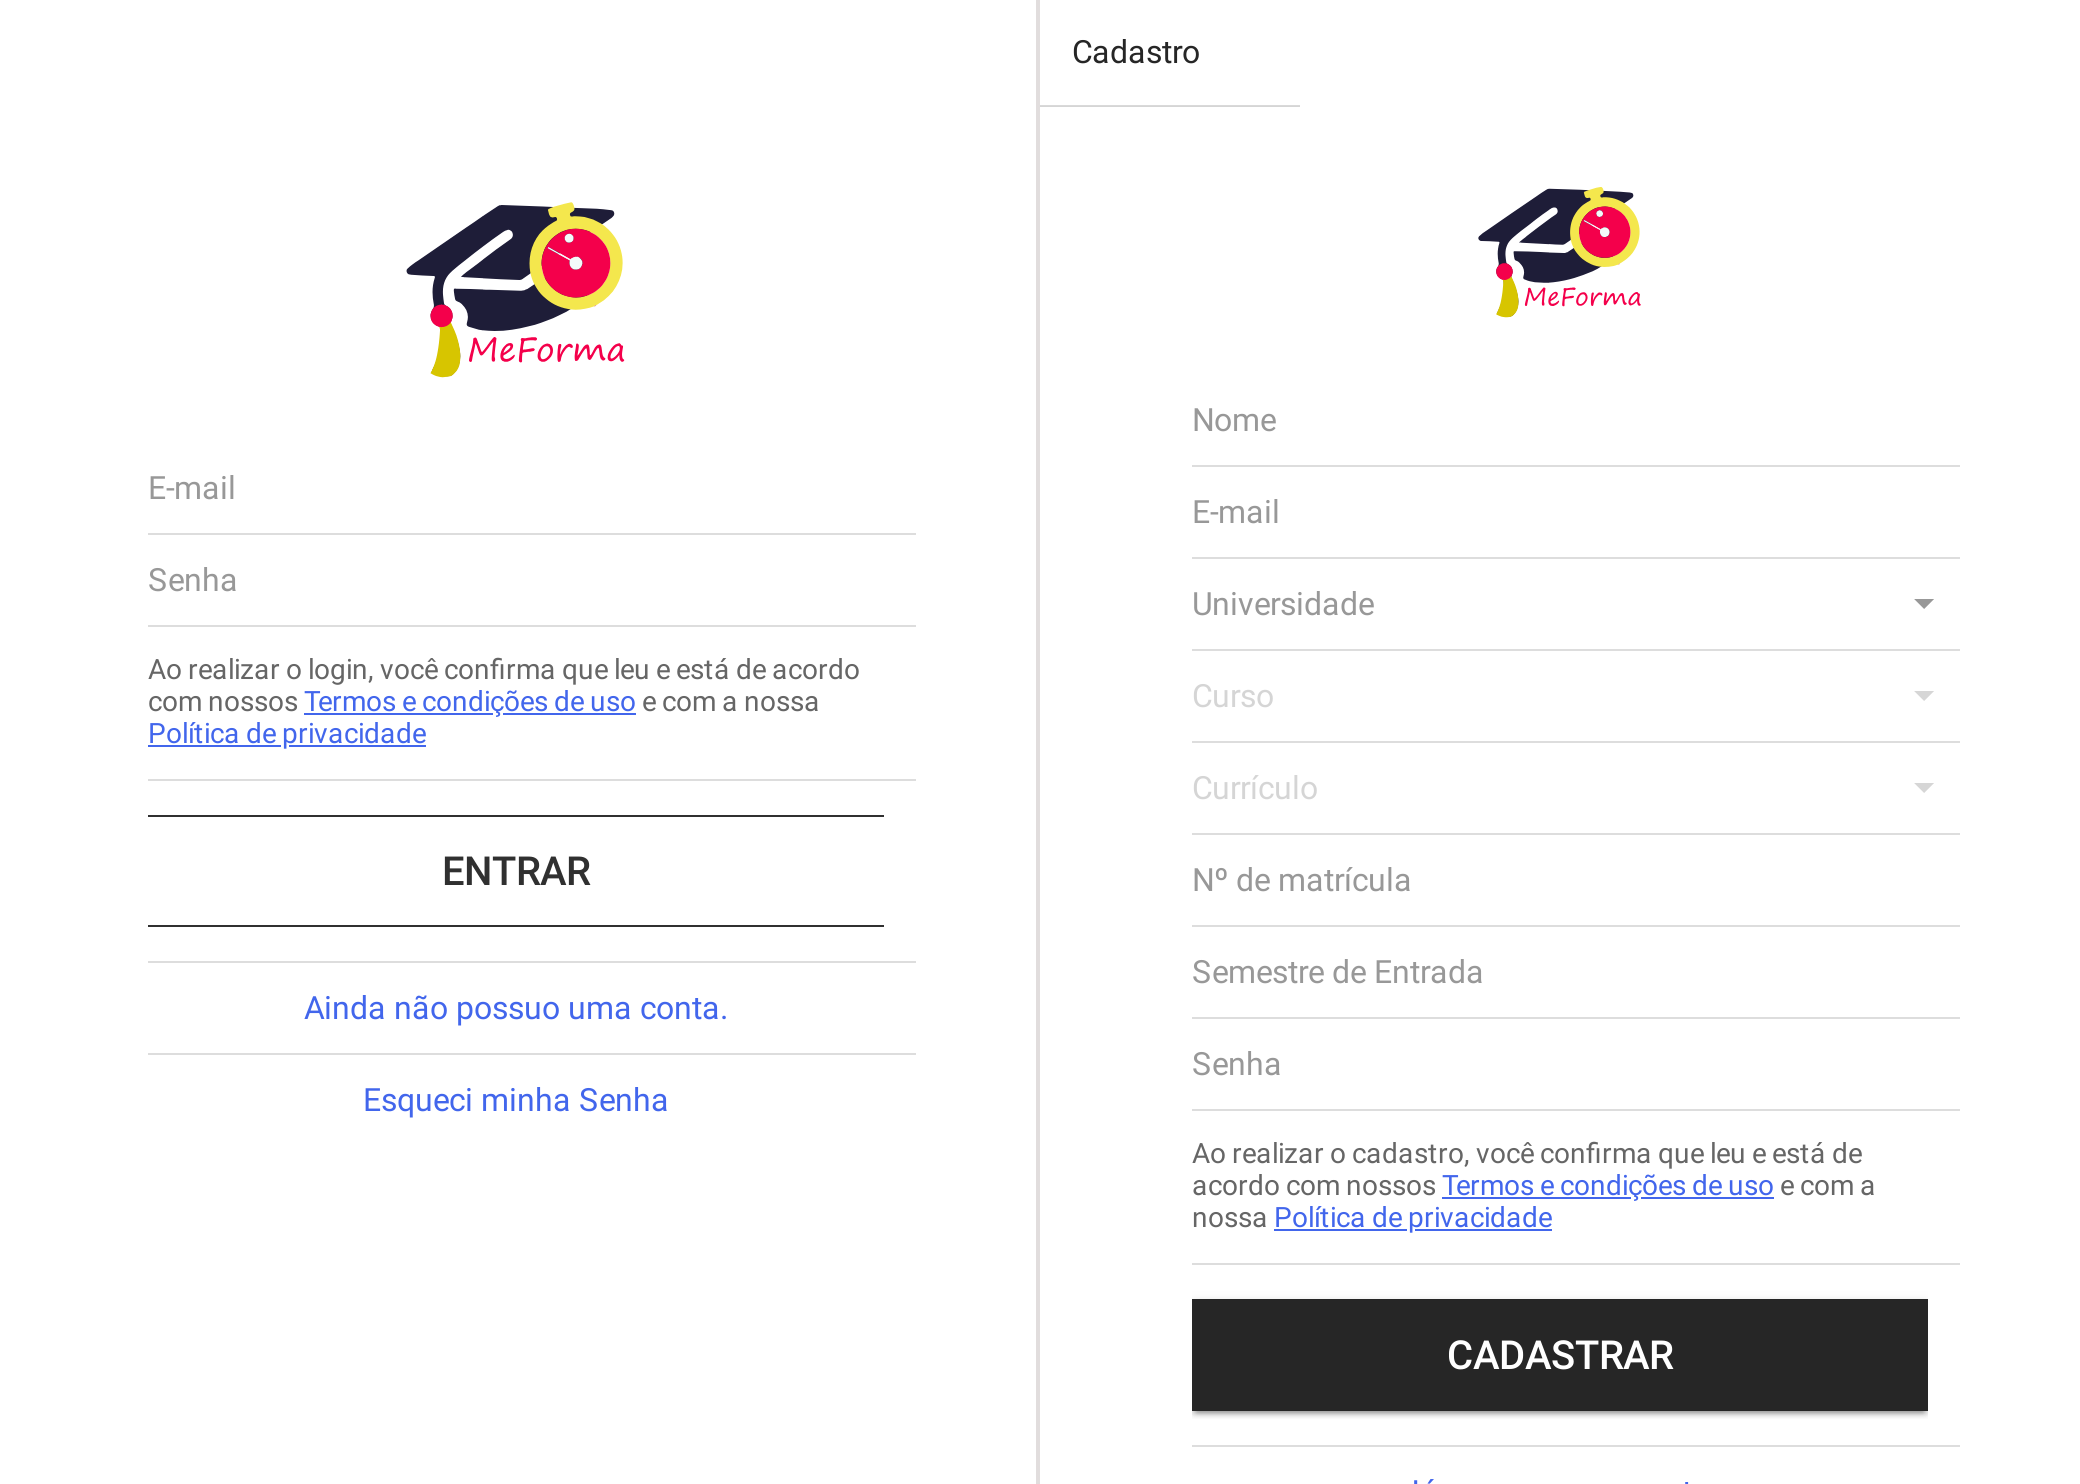
\includegraphics[scale=0.25]{pics/c3/1-login.png}
	   \caption{Tela de Login e Tela de Cadastro}
	   \label{login}
\end{figure}

\subsection{Visualização de Conclusão de Curso}
Após o login bem sucedido, o usuário é direcionado para a tela inicial do sistema, onde ele pode acompanhar a porcentagem de conclusão de cada elemento requisitado para conclusão do curso, além da porcentagem total de conclusão (Figura~\ref{completude}).
\begin{figure}[H]
	   \centering
	   		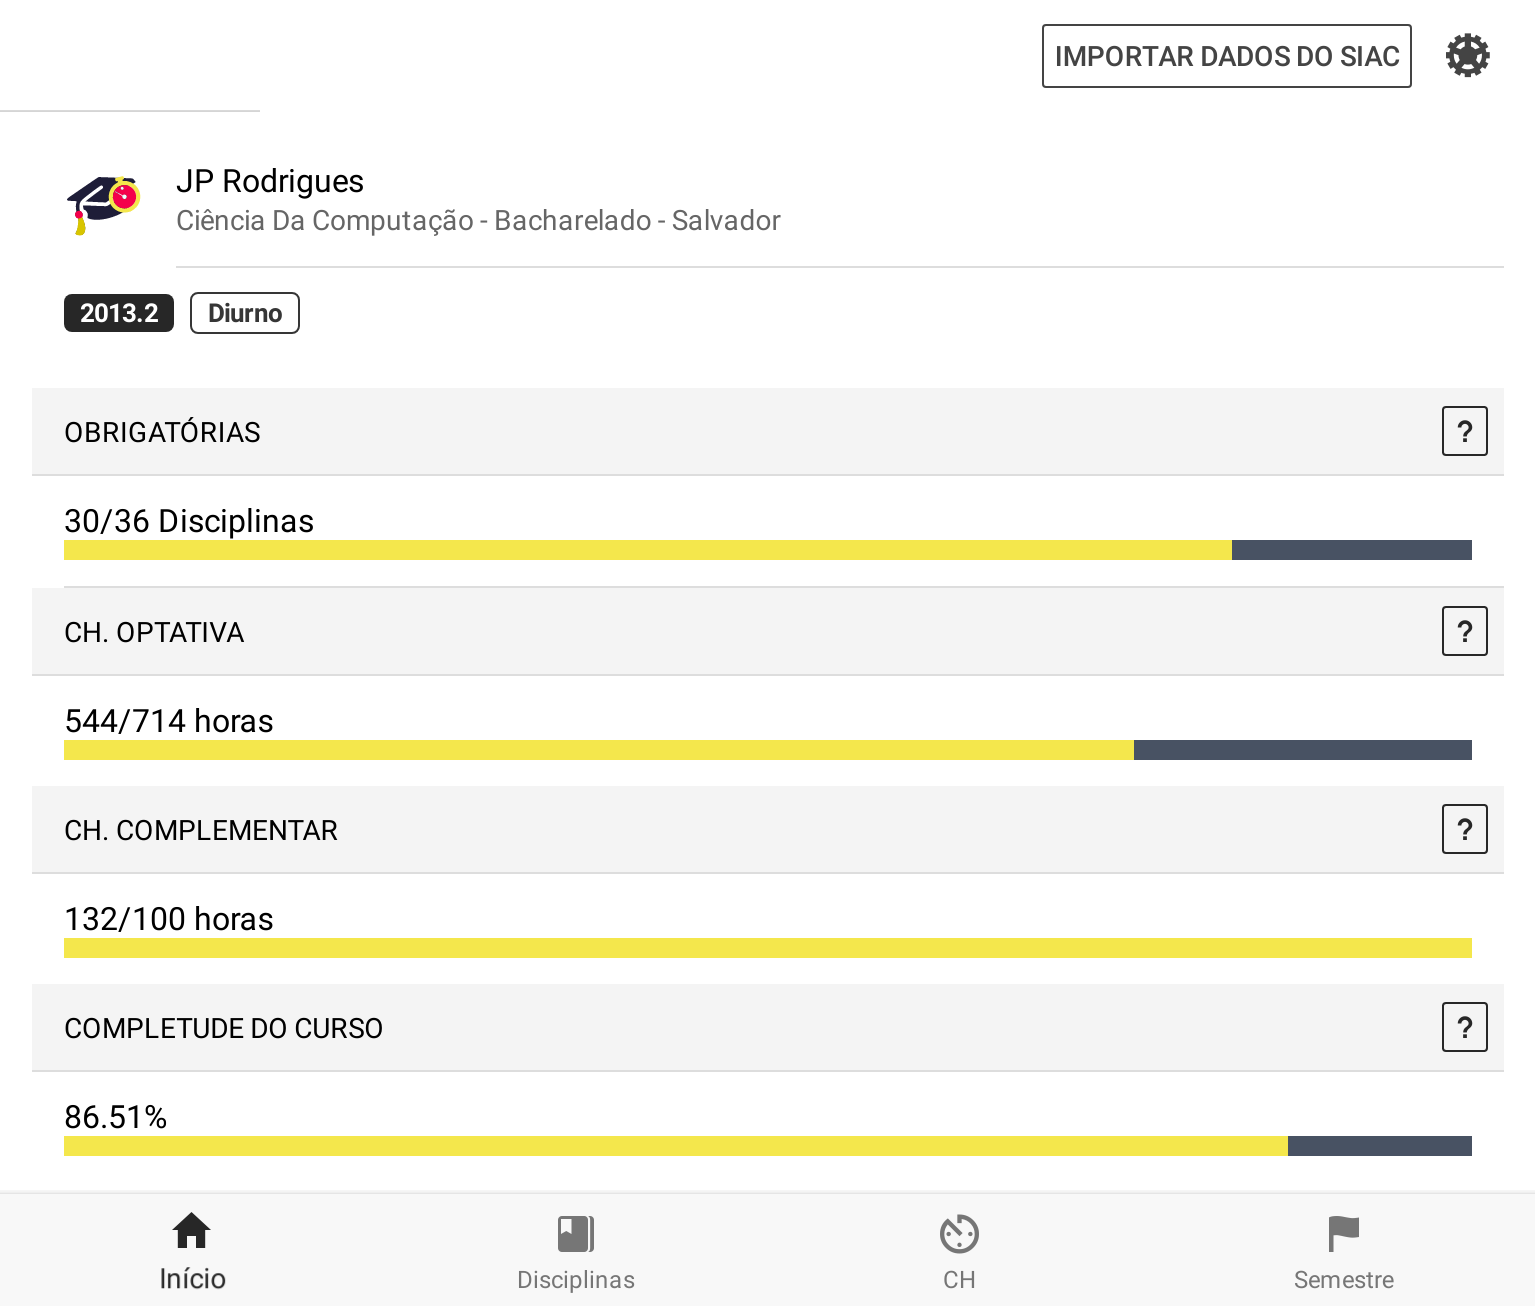
\includegraphics[scale=0.25]{pics/c3/3-completude.png}
	   \caption{Tela de completude do curso.}
	   \label{completude}
\end{figure}

\subsection{Seleção de Disciplinas Concluídas}
\label{disciplinas_tela}
Fundamental para o cumprimento do objetivo do sistema, essa é uma tela acessada ao clicar-se em ‘Disciplinas’, segunda opção disponível no menu do usuário.  A tela é secionada em duas listas de itens que representam as disciplinas, as ‘Obrigatórias’ e as ‘Optativas’ (Figura~\ref{disciplines}). Cada item é acompanhado por uma caixa de seleção (checkbox), a qual, ao ser selecionada, registra aquela disciplina como concluída e, ao ser desmarcada, remove o registro de que aquela disciplina foi concluída e, assim, a depender da ação executada pelo usuário, uma disciplina é incluída ou removida do cálculo de conclusão de curso.

\begin{figure}[H]
	   \centering
	   		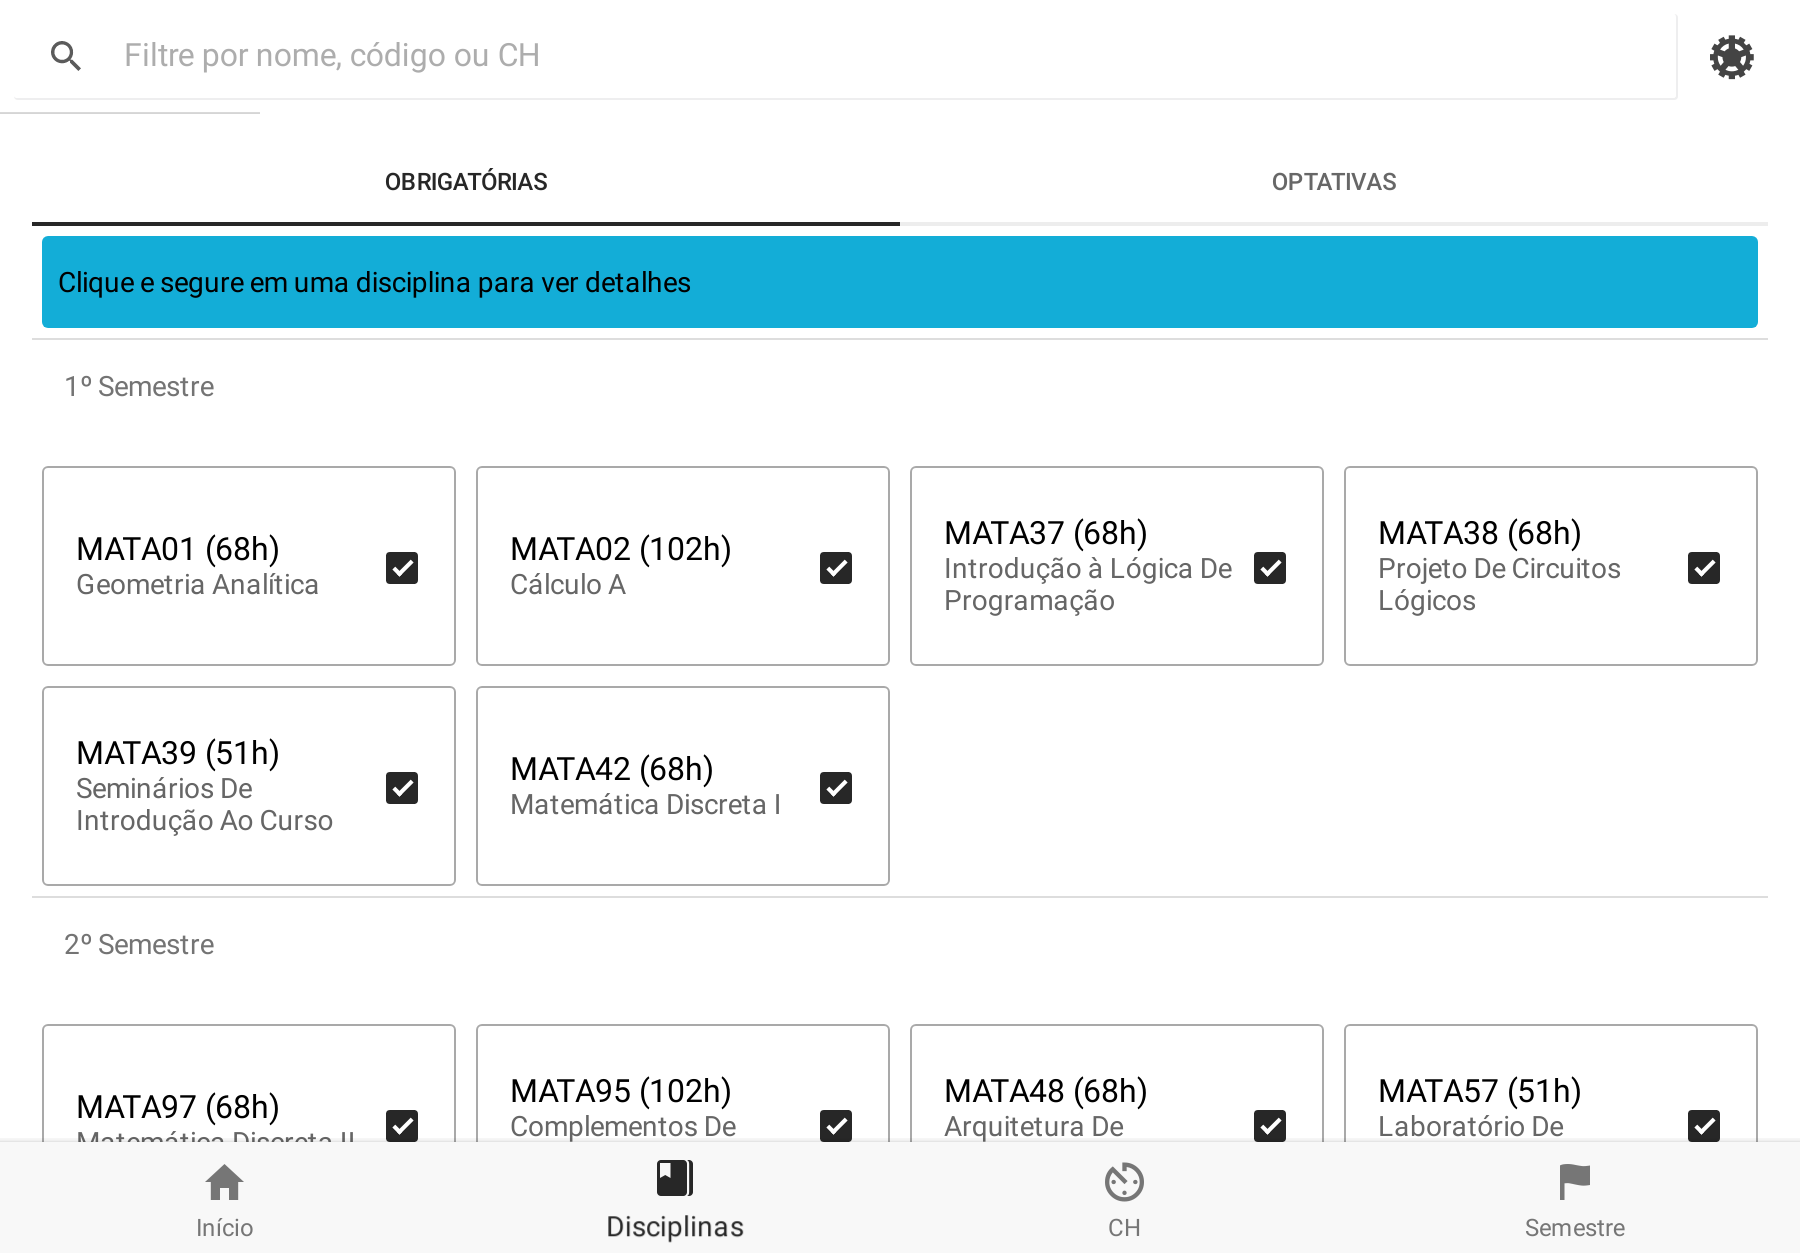
\includegraphics[scale=0.25]{pics/c3/5-disciplines.png}
	   \caption{Tela de disciplinas do curso.}
	   \label{disciplines}
\end{figure}

As disciplinas obrigatórias são segmentadas por semestre (Figura~\ref{disciplines}), a fim de facilitar a identificação de uma disciplina na lista e orientar o usuário com relação à conclusão de um semestre.
As disciplinas optativas exibidas são aquelas sugeridas pelo curso e são exibidas sem categorização (Figura~\ref{optionals}).

\begin{figure}[H]
	   \centering
	   		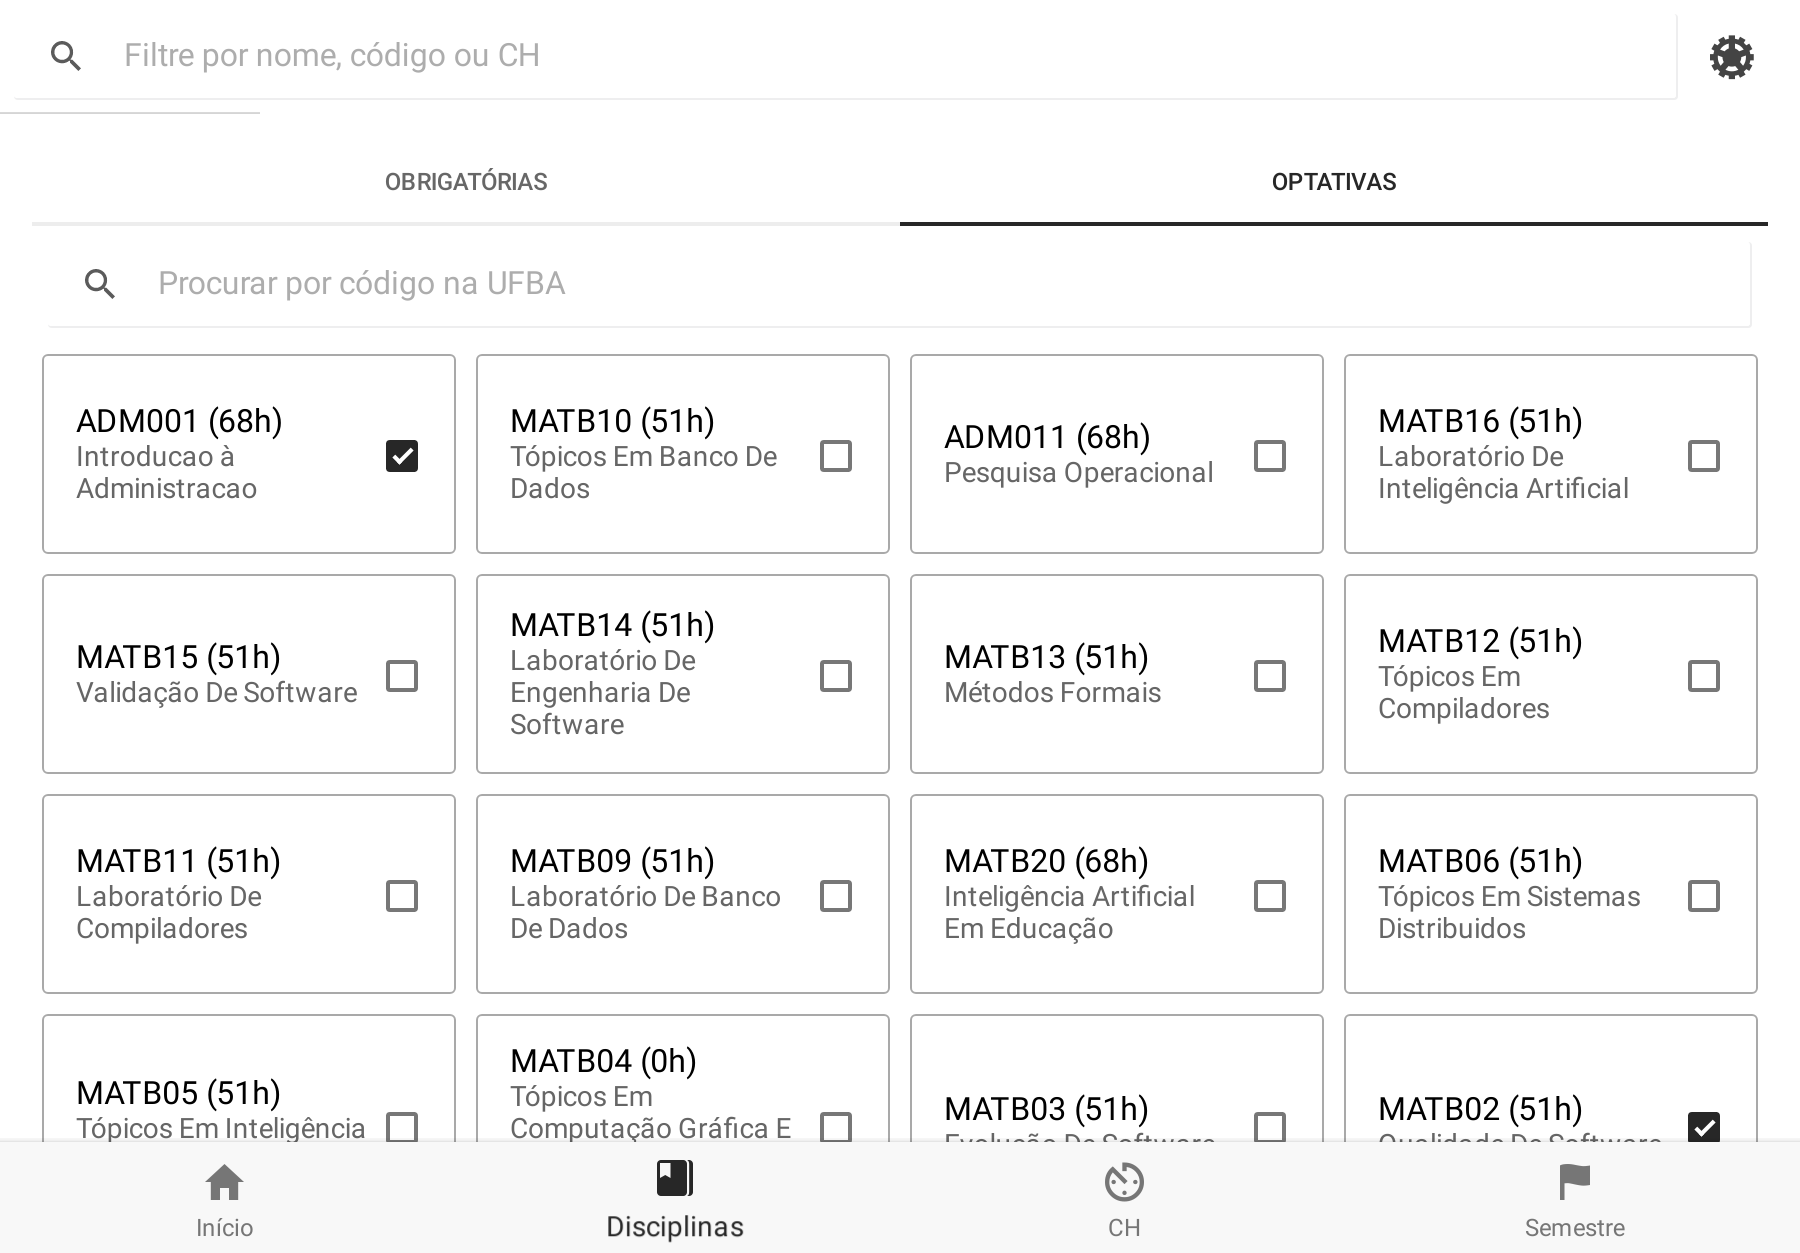
\includegraphics[scale=0.25]{pics/c3/6-optionals.png}
	   \caption{Tela de disciplinas optativas sugeridas pelo curso.}
	   \label{optionals}
\end{figure}

Na seção de disciplinas optativas, o usuário pode buscar uma disciplina em toda a lista de disciplinas do MeForma através do código da disciplina.

O usuário pode ainda buscar uma disciplina por nome, código ou carga horária utilizando a ‘caixa de pesquisa do curso’ localizada no topo da página, mas diferente do campo de busca de optativas, essa caixa de pesquisa só retorna disciplinas que estejam dentre as obrigatórias e optativas oferecidas pelo curso.

Ainda nessa tela, quando o usuário clica e segura em um item, é exibida uma janela no estilo “modal” que exibe a lista completa de pré-requisitos e dependências daquela disciplina.

Na versão web do MeForma, quando o ponteiro do mouse está sob a representação de uma disciplina, os cartões das disciplinas que estão conectadas a ela são destacados. 

A conexão entre disciplinas pode ser do tipo pré-requisito ou do tipo dependência. Sejam A e B duas disciplinas. Se a disciplina A é pré-requisito para a disciplina B, implica que a disciplina B tem a disciplina A como dependência. Graficamente, se uma disciplina A é pré-requisito para uma disciplina B, a disciplina B é destacada na cor verde quando o ponteiro do mouse está sob a disciplina A, por outro lado, quando o ponteiro do mouse está sob a disciplina B, a disciplina A é destacada em tons de vermelho. A Figura~\ref{highlight} mostra a interação do usuário com a disciplina MATA40, que provoca o destaque da disciplina MATA42 como pré-requisito e da disciplina MATA49 como dependente.

O destaque dos pré-requisitos e dependências por cor, tem a finalidade de orientar o usuário com relação à evolução do curso conforme as disciplinas são concluídas.

\begin{figure}[H]
	   \centering
	   		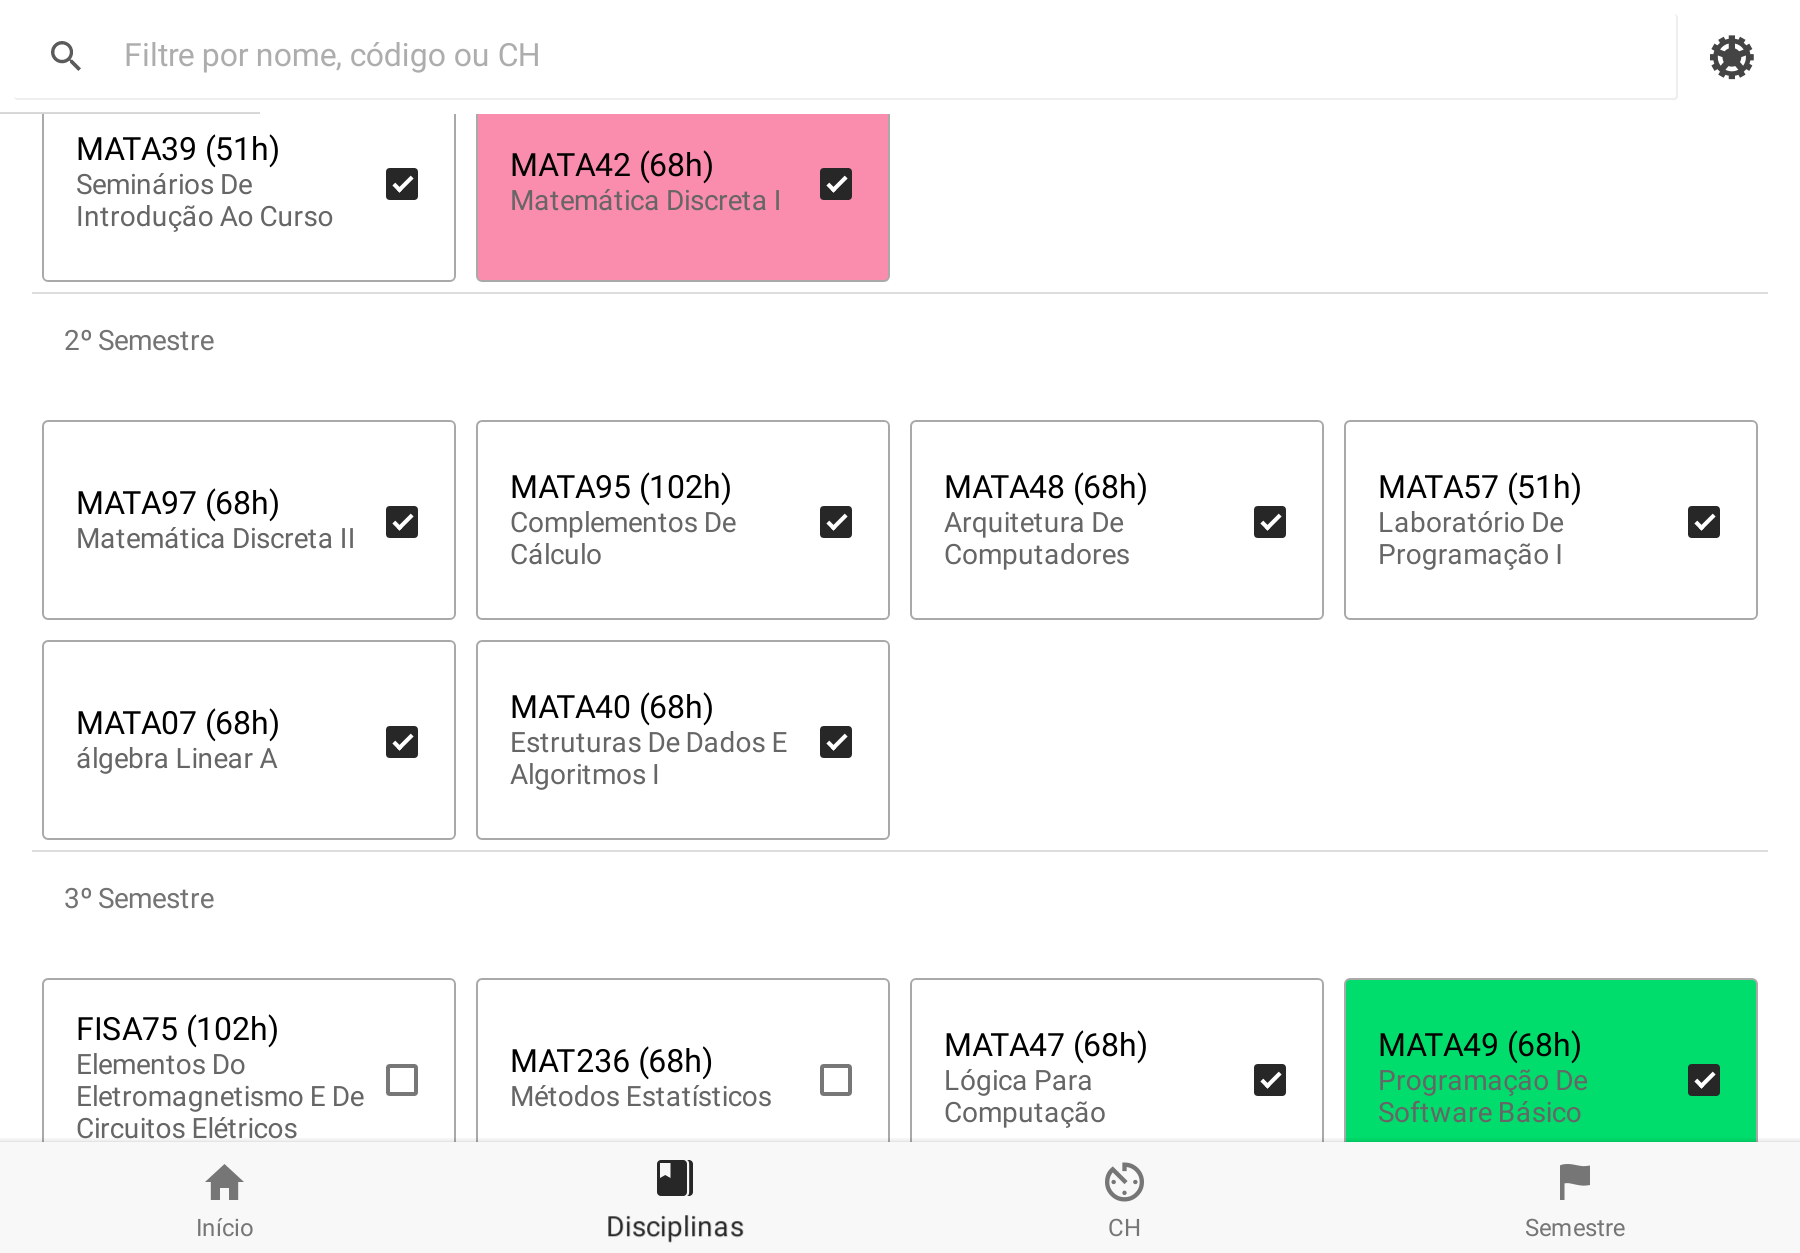
\includegraphics[scale=0.25]{pics/c3/7-highlight.png}
	   \caption{Dependências e pré-requisitos em destaque para a disciplina MATA40.}
	   \label{highlight}
\end{figure}
\subsection{Cadastro de Carga Horária Extra}
A carga horária extra possui três classificações distintas no MeForma2. São elas: optativas, complementares e livres. Cada currículo de curso tem um valor mínimo específico para esses tipos de carga horária. Esse valor também pode ser nulo.

Na tela de carga horária, terceira opção no menu do usuário, os aproveitamentos são secionados de acordo com sua classificação (Figura~\ref{ch}). Ao usuário é apresentado um botão de adição que, ao ser clicado, exibe o formulário de registro de carga horária (Figura~\ref{createch}), o qual exige que o usuário insira a quantidade de horas que foi aproveitada, como essas horas foram aproveitadas,  qual o tipo de carga horária a ser aproveitada (optativa, complementar ou livre) e permite que o usuário deixe um comentário sobre aquele aproveitamento. O registro de um aproveitamento de carga horária o inclui automaticamente no cálculo de conclusão de curso.

Os aproveitamentos são representados por um cartão que exibe como o mesmo se deu, a quantidade de horas correspondentes, e o comentário adicionado pelo usuário, além de oferecer ao usuário as opção de editar e de excluir o aproveitamento. As opções de editar e excluir servem como ferramentas para que os usuários possam se recuperar de erros.

\begin{figure}[H]
	   \centering
	   		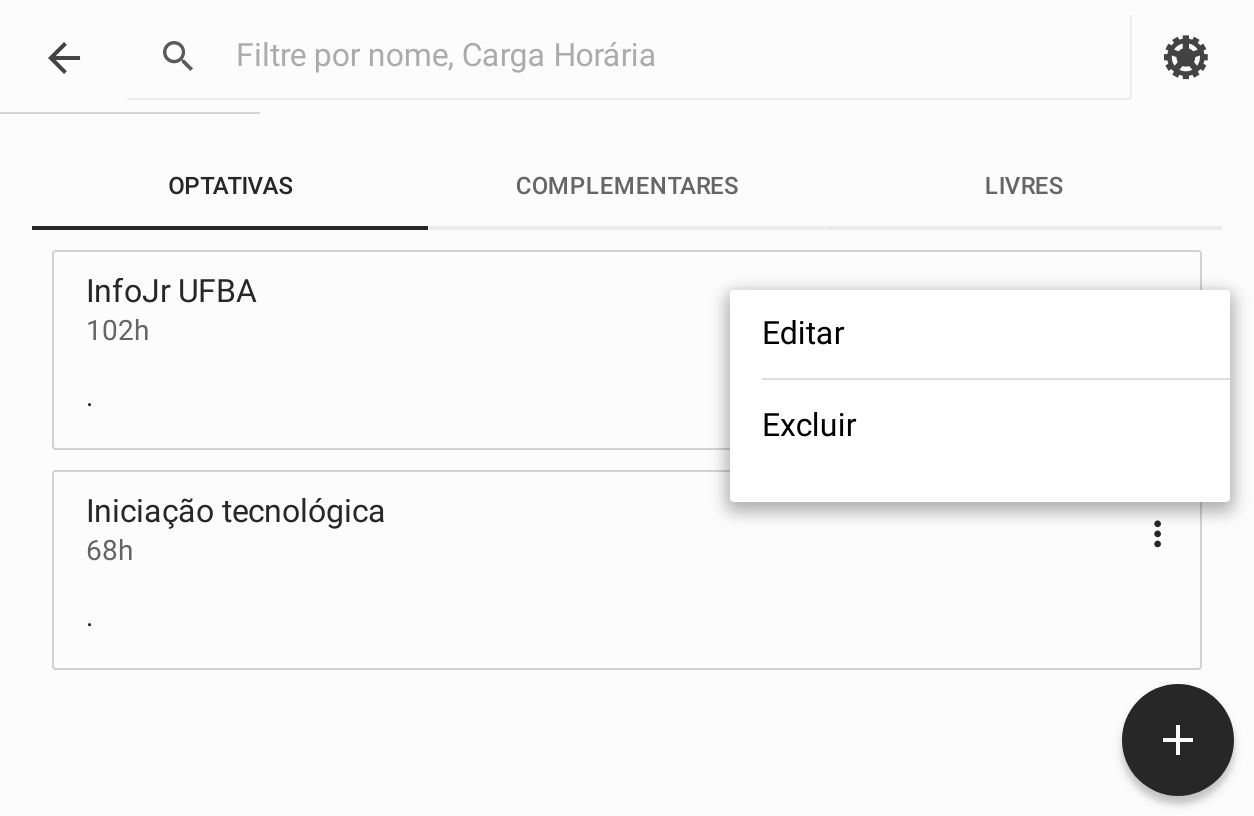
\includegraphics[scale=0.25]{pics/c3/8-ch.png}
	   \caption{Tela de exibição de carga horária.}
	   \label{ch}
\end{figure}

\begin{figure}[H]
	   \centering
	   		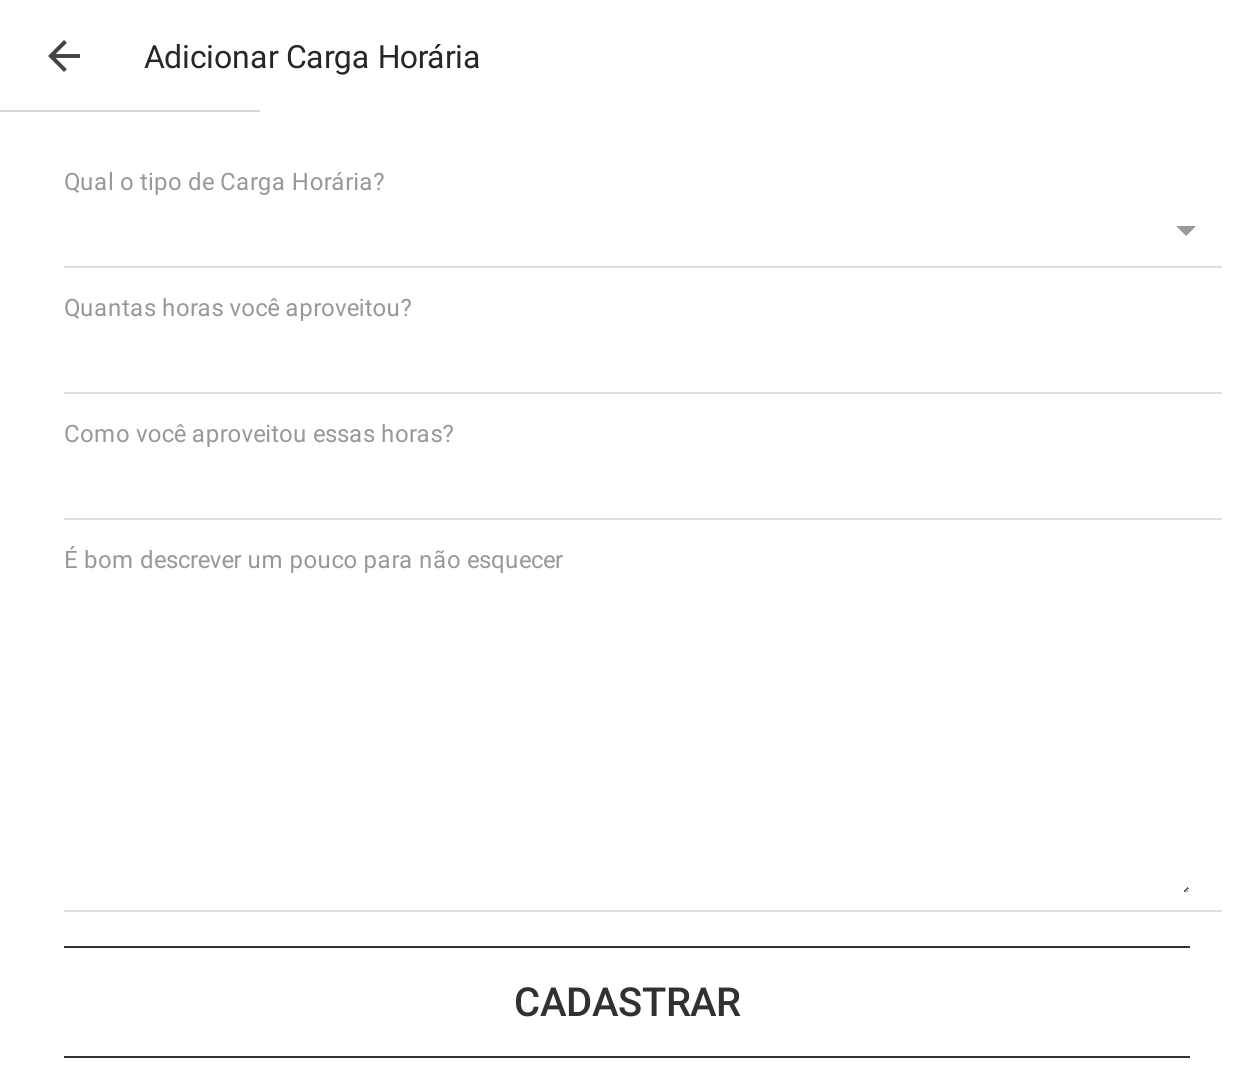
\includegraphics[scale=0.25]{pics/c3/9-createch.png}
	   \caption{Tela de criação de carga horária.}
	   \label{createch}
\end{figure}

\subsection{Registro de Semestre}
O registro de semestre é importante para que o usuário possa controlar seu número de faltas em uma disciplina, além de permitir que ele acompanhe seu avanço no curso. 

O primeiro contato que o usuário tem com os semestres é quando ele acessa a quarta opção do menu do usuário, ``Semestre''. A tela de semestre exibe o semestre mais recente que o usuário registrou e as disciplinas que compõem aquele semestre e, para cada disciplina, o painel de controle de faltas. A tela também exibe as opções de ver todos os semestres e de cadastrar um novo semestre (Figura~\ref{semester}).
\begin{figure}[H]
	   \centering
	   		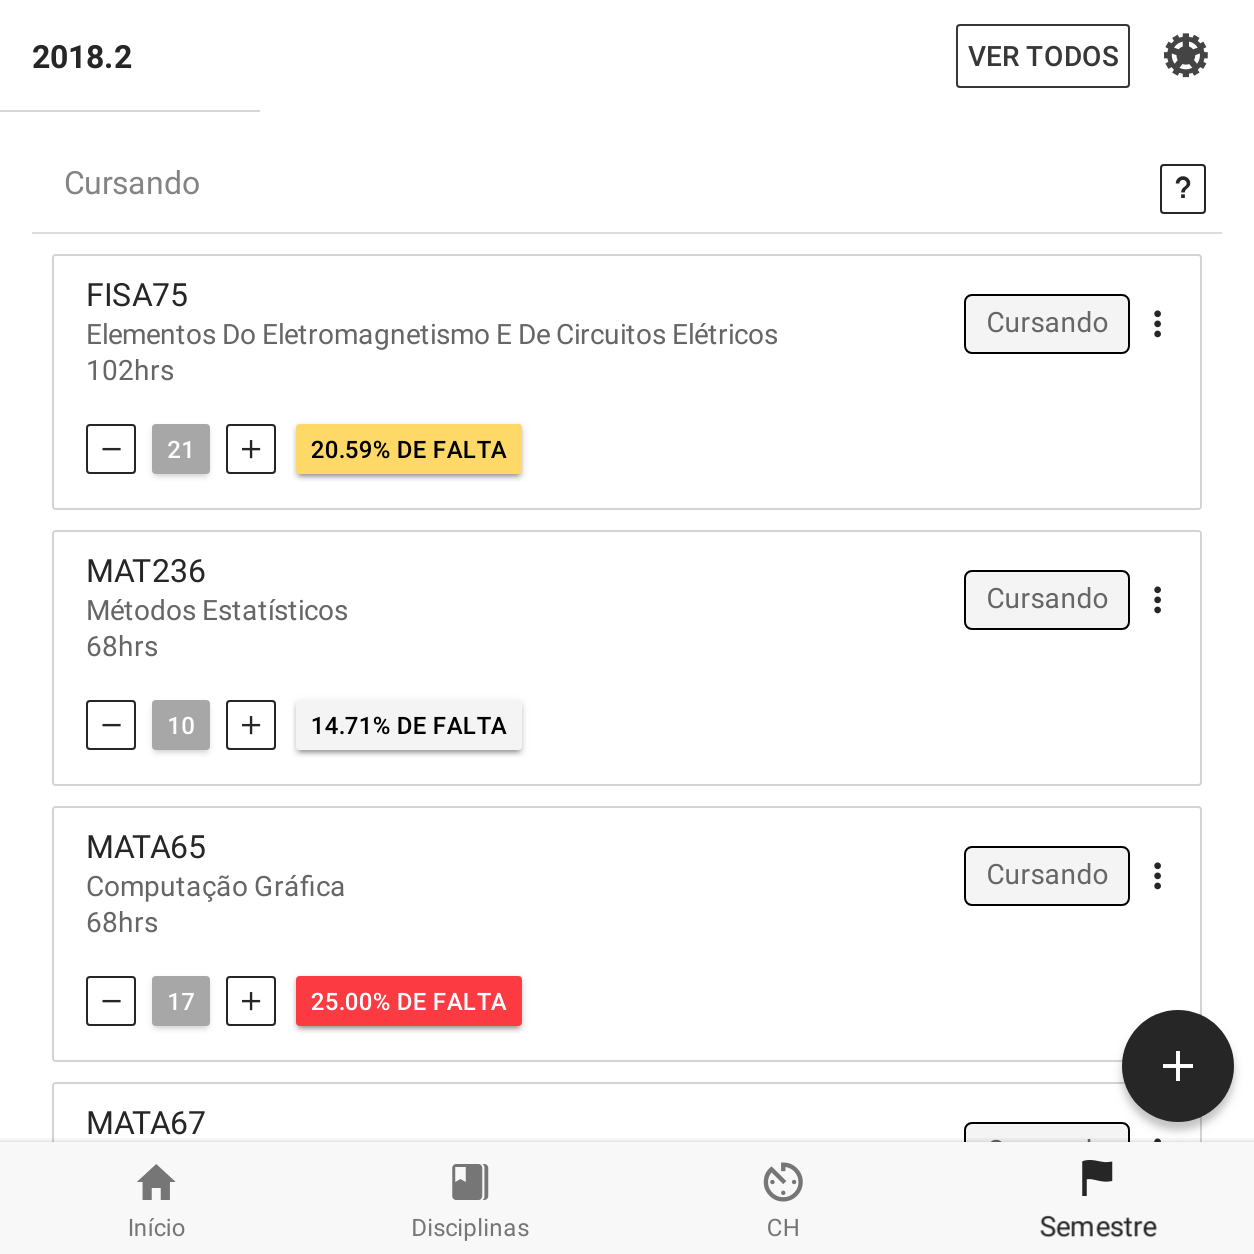
\includegraphics[scale=0.25]{pics/c3/10-semester.png}
	   \caption{Tela de exibição de semestre.}
	   \label{semester}
\end{figure}

A opção de cadastrar um novo semestre exibe uma tela que solicita o código de identificação do semestre que o usuário deseja cadastrar , o qual, após ser inserido, libera a lista de disciplinas do curso para que o usuário possa selecionar as que correspondem àquele semestre (Figura~\ref{newsemester}.

\begin{figure}[H]
	   \centering
	   		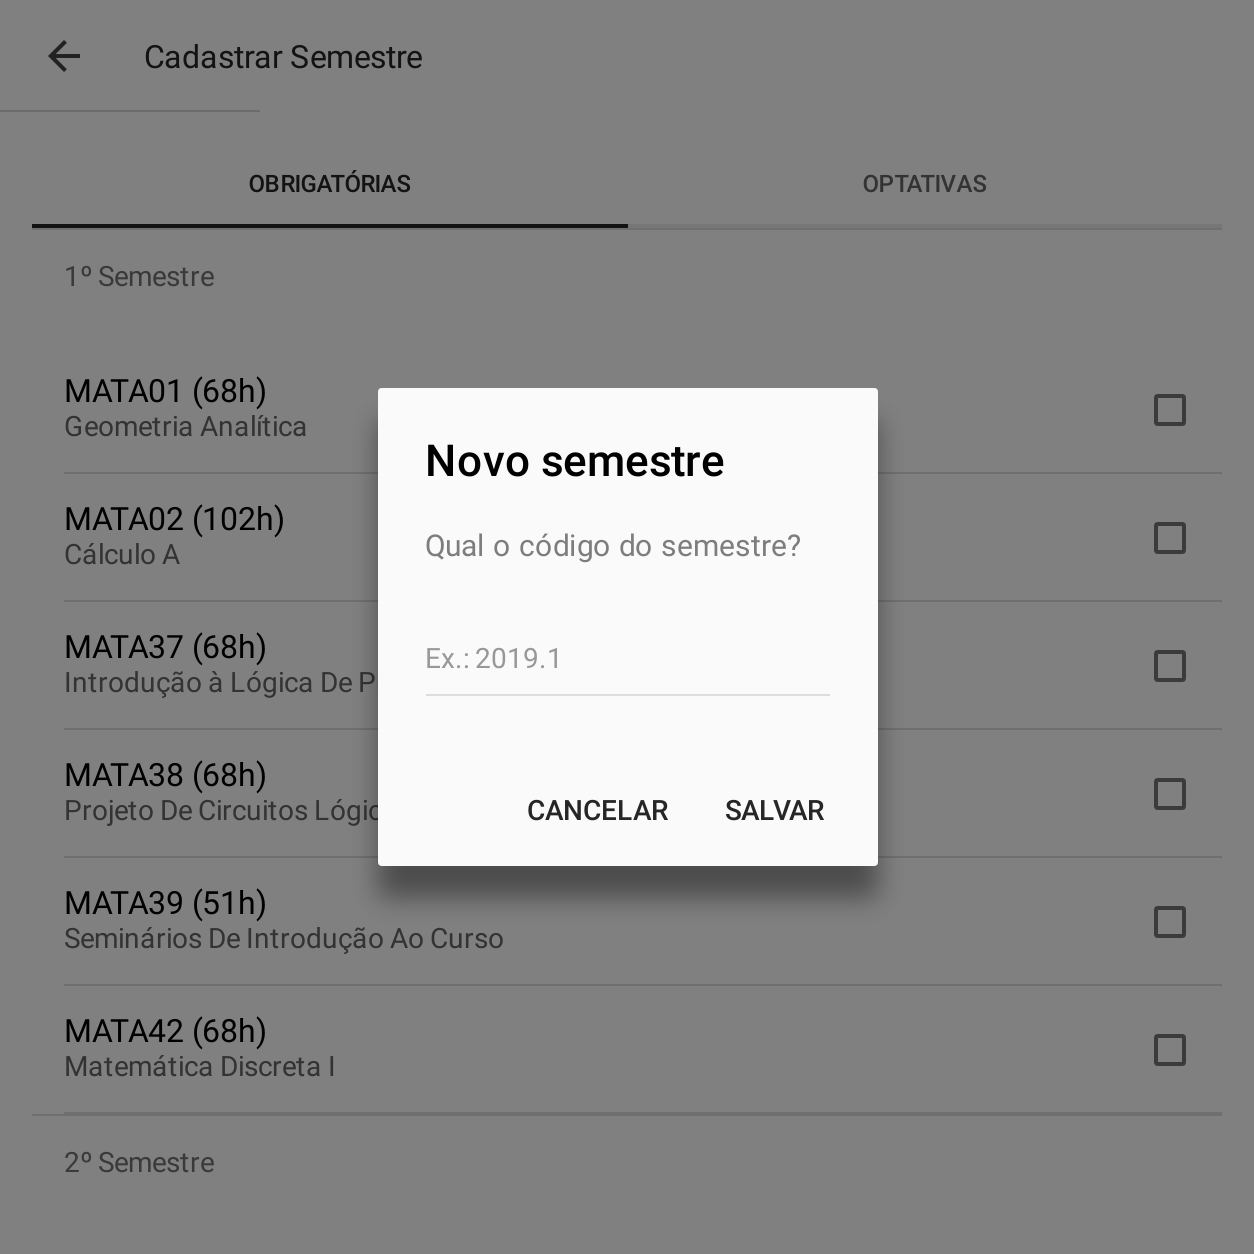
\includegraphics[scale=0.25]{pics/c3/11-newsemester.png}
	   \caption{Tela de cadastro de semestre.}
	   \label{newsemester}
\end{figure}

A opção ``Ver Todos'' exibe uma lista com todos os semestres cadastrados no sistema pelo usuário e as opções de editar um semestre (que implica na possibilidade de alterar o código de identificação), alterar disciplinas, e excluir semestre.

Nas telas de ``Semestre atual'' e de ``Todos os semestres'', cada disciplina é apresentada graficamente como um cartão que oferece ao usuário dois botões responsáveis por incrementar e decrementar as faltas naquela disciplina. As faltas são alteráveis em qualquer tempo. A funcionalidade de controle de faltas é exibida na figura~\ref{semester}.

\subsection{Recuperação de Dados do Siac Web}
O Siac é um portal onde os estudantes da UFBA podem acompanhar dados referentes à matrícula semestral. Através desse portal o MeForma é capaz de obter automaticamente os dados sobre as disciplinas optativas e obrigatórias cursadas pelo estudante necessários para o gráfico de conclusão. A Figura \ref{siac} mostra como o estudante pode recuperar os dados do Siac.

\begin{figure}[H]
	   \centering
	   		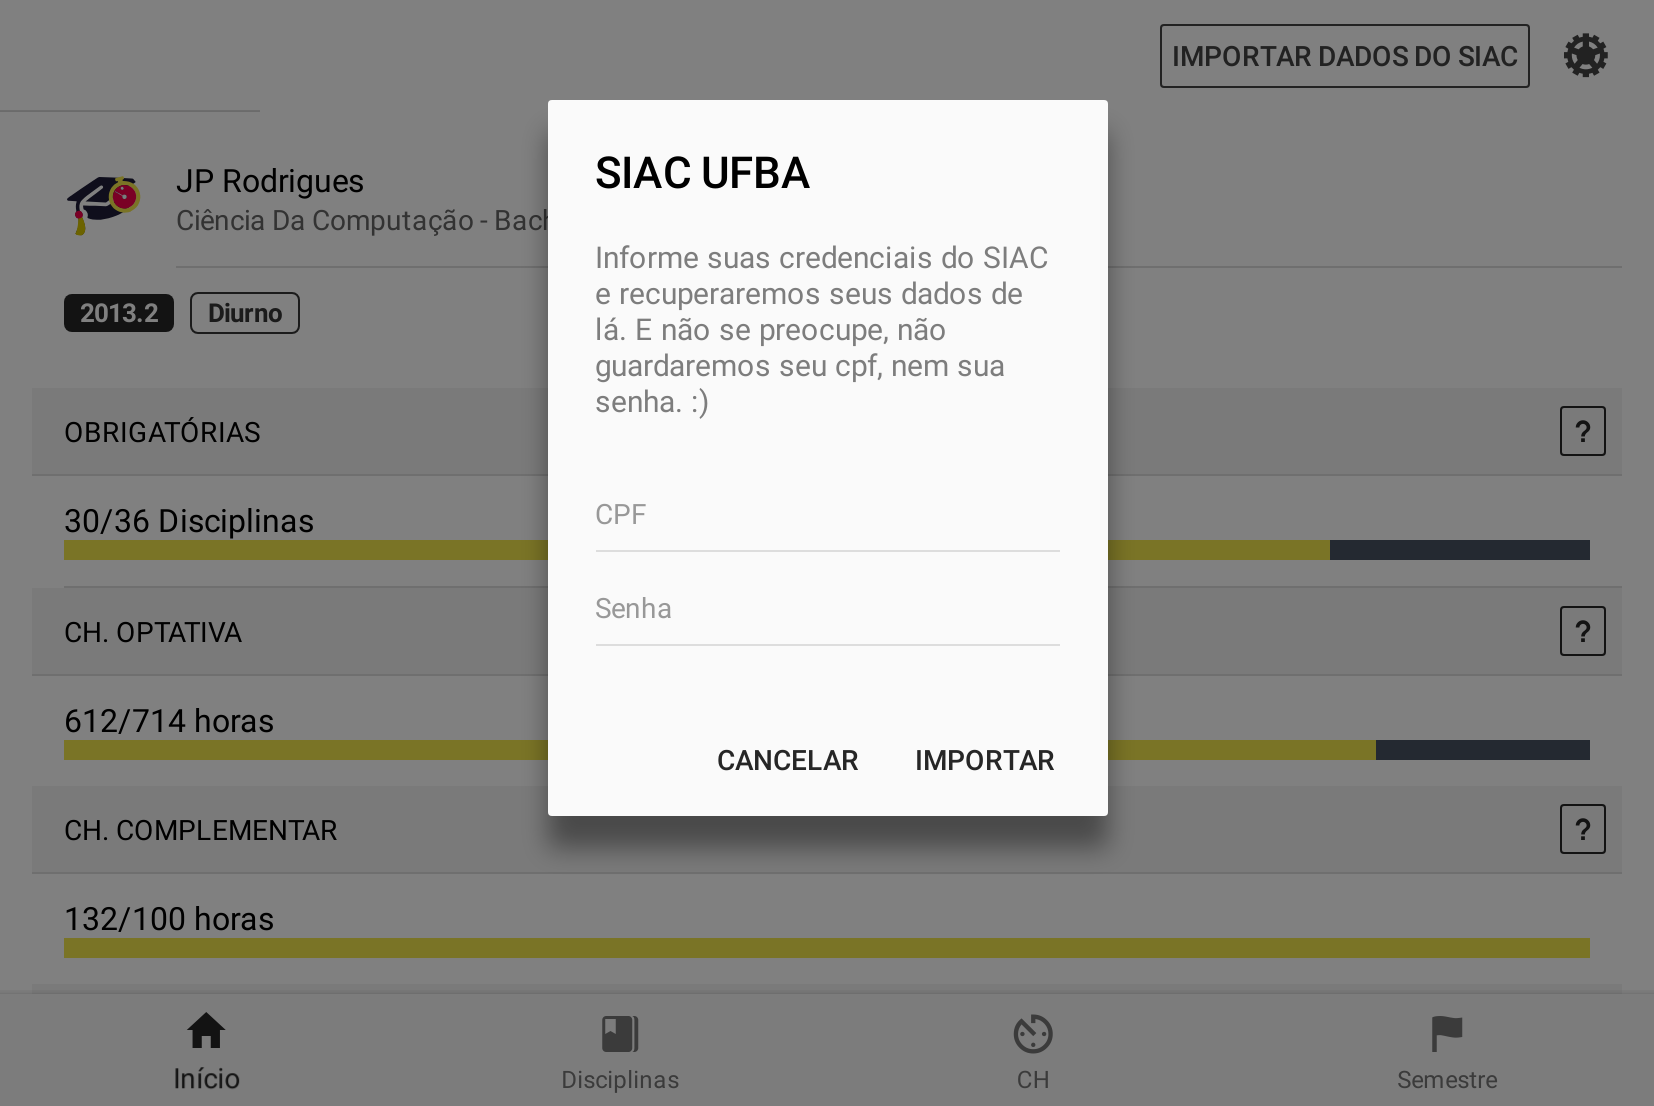
\includegraphics[scale=0.25]{pics/c3/13-siac.png}
	   \caption{Tela de recuperação de dados do Siac.}
	   \label{siac}
\end{figure}

\subsection{Porcentagem de aprovação das disciplinas}

Quando o estudante recupera seus dados do Siac, a tela de disciplinas do curso passa a exibir a porcentagem de aprovação de cada disciplina, a fim de ajudar o estudante a planejar o conjunto de disciplinas que ele vai cursar por semestre.

A porcentagem de aprovação é acompanhada por uma barra de status que indica através das cores vermelho, amarelo e azul a categoria da disciplina com relação à porcentagem de aprovações. A cor vermelho indica um número criticamente baixo de aprovações, a cor amarelo indica um número baixo de aprovações, a cor azul indica um número satisfatório de aprovações. A Figura \ref{percentages} exibe a tela de disciplinas do curso com as suas respectivas porcentagens de aprovação.

O cálculo de porcentagem de aprovação considera apenas os estudantes cadastrados no MeForma2 que estão cursando o mesmo currículo de curso que o usuário que está acessando o sistema e que recuperaram seus dados do Siac. Esses limites foram impostos para aumentar a confiabilidade dos números gerados.

Um detalhe importante sobre a porcentagem de aprovação é que ela diz respeito à amostra de estudantes que estão cadastrados no MeForma2, desse modo, para que o valor seja próximo da realidade do currículo do curso, o ideal é que muitos estudantes tenham recuperado seus dados do Siac.


\begin{figure}[H]
	   \centering
	   		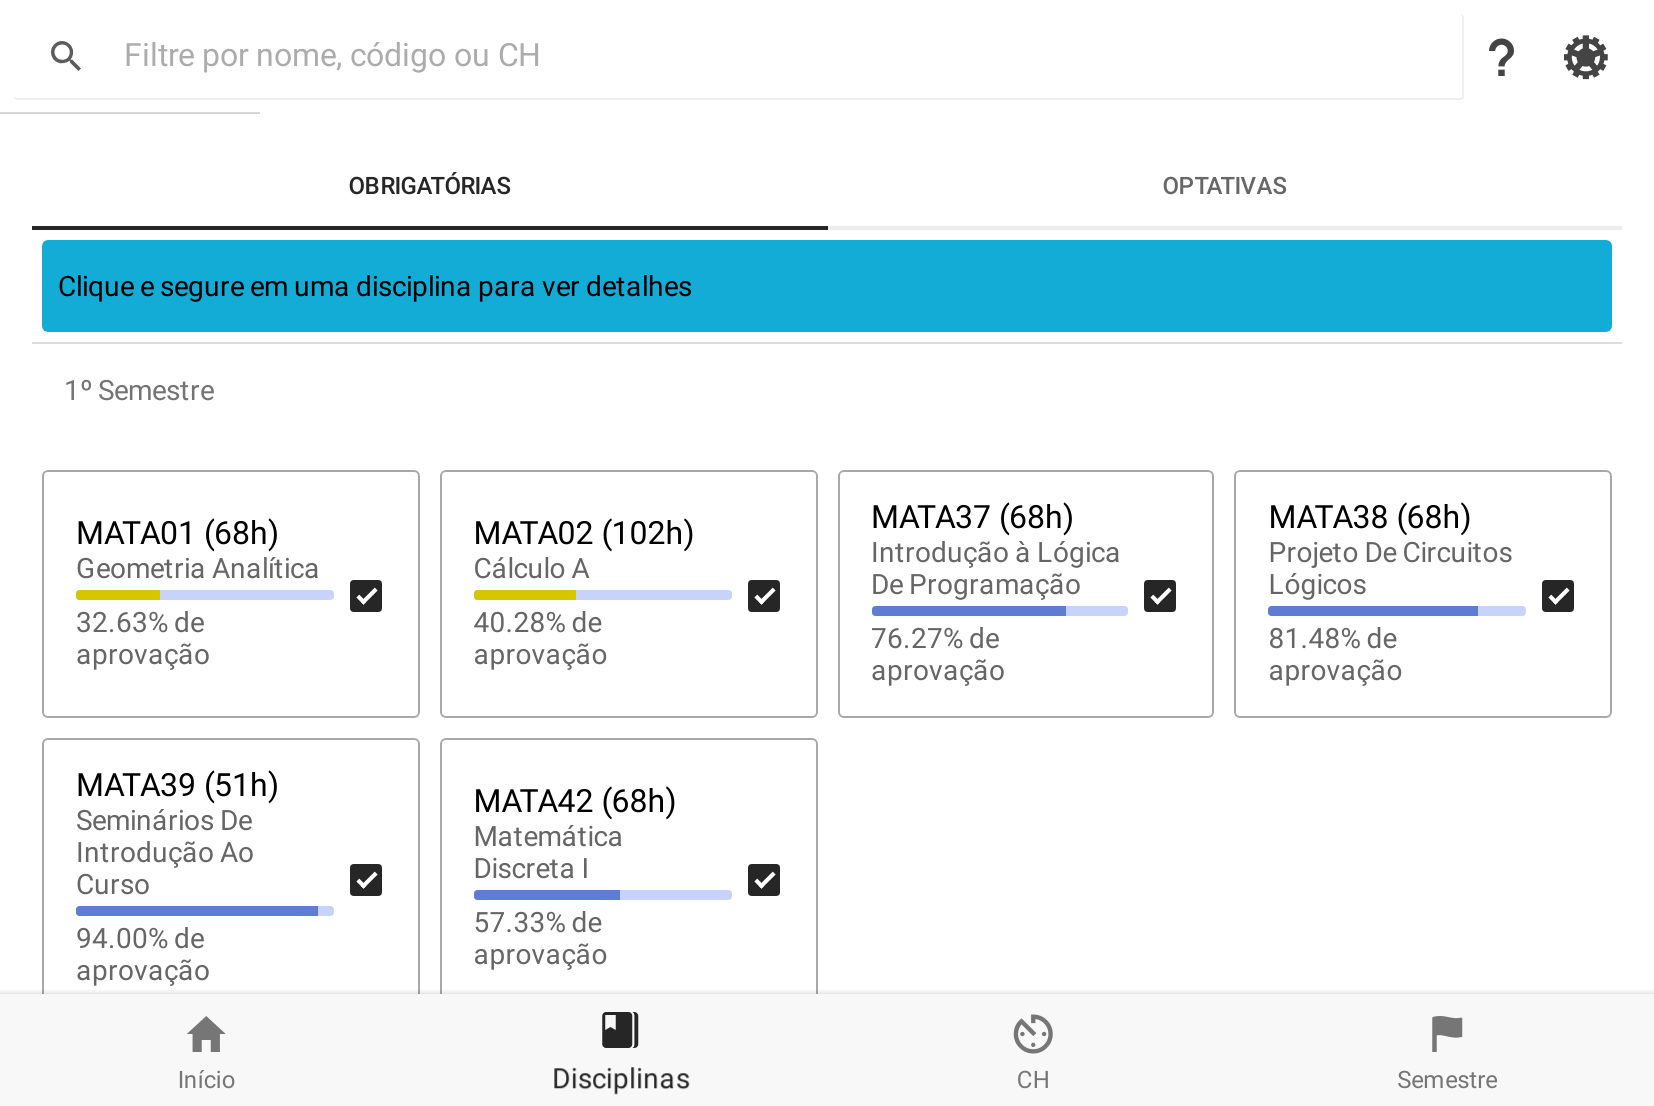
\includegraphics[scale=0.25]{pics/c3/14-percentage.png}
	   \caption{Tela de disciplinas do curso com porcentagem de aprovação.}
	   \label{percentages}
\end{figure}

\section{Painel de Acompanhamento dos Cursos}

O Painel de Acompanhamento dos Cursos - MFPAC é uma sequência de telas do MeForma2 disponível apenas para gestores dos cursos de graduação cadastrados no sistema. Com o MFPAC o gestor pode analisar os dados gerados pela utilização do MeForma2 por parte dos estudantes de cada currículo dos cursos que ele gerencia. A seguir serão apresentadas as principais telas que compõem o painel.

\subsection{Resumo de desempenho nas disciplinas}

A tela de resumo de desempenho das disciplinas exibe 5 gráficos que apresentam as 10 disciplinas com maior porcentagem de aprovação, as 10 disciplinas com maior porcentagem de reprovação, as 10 disciplinas com maior porcentagem de desistência, as 10 disciplinas com maior porcentagem de trancamento e as 10 disciplinas com maior porcentagem de reprovações por falta. Os dados podem ser filtrados por curso, currículo e período. A Figura \ref{charts} exibe a tela de resumo de desempenho das disciplinas para o curso de Ciência da Computação da UFBA referentes aos estudantes com currículo 2013.2 para o período de 2010.2 a 2018.2.

As porcentagens são calculadas apenas com os estudantes que recuperaram seus dados do Siac, a fim de melhorar a confiabilidade dos números. Contudo, vale ressaltar que os números são referentes a uma amostra que se aproxima dos valores reais conforme aumenta a quantidade de estudantes cadastrados no MeForma2.

\begin{figure}[H]
	   \centering
	   		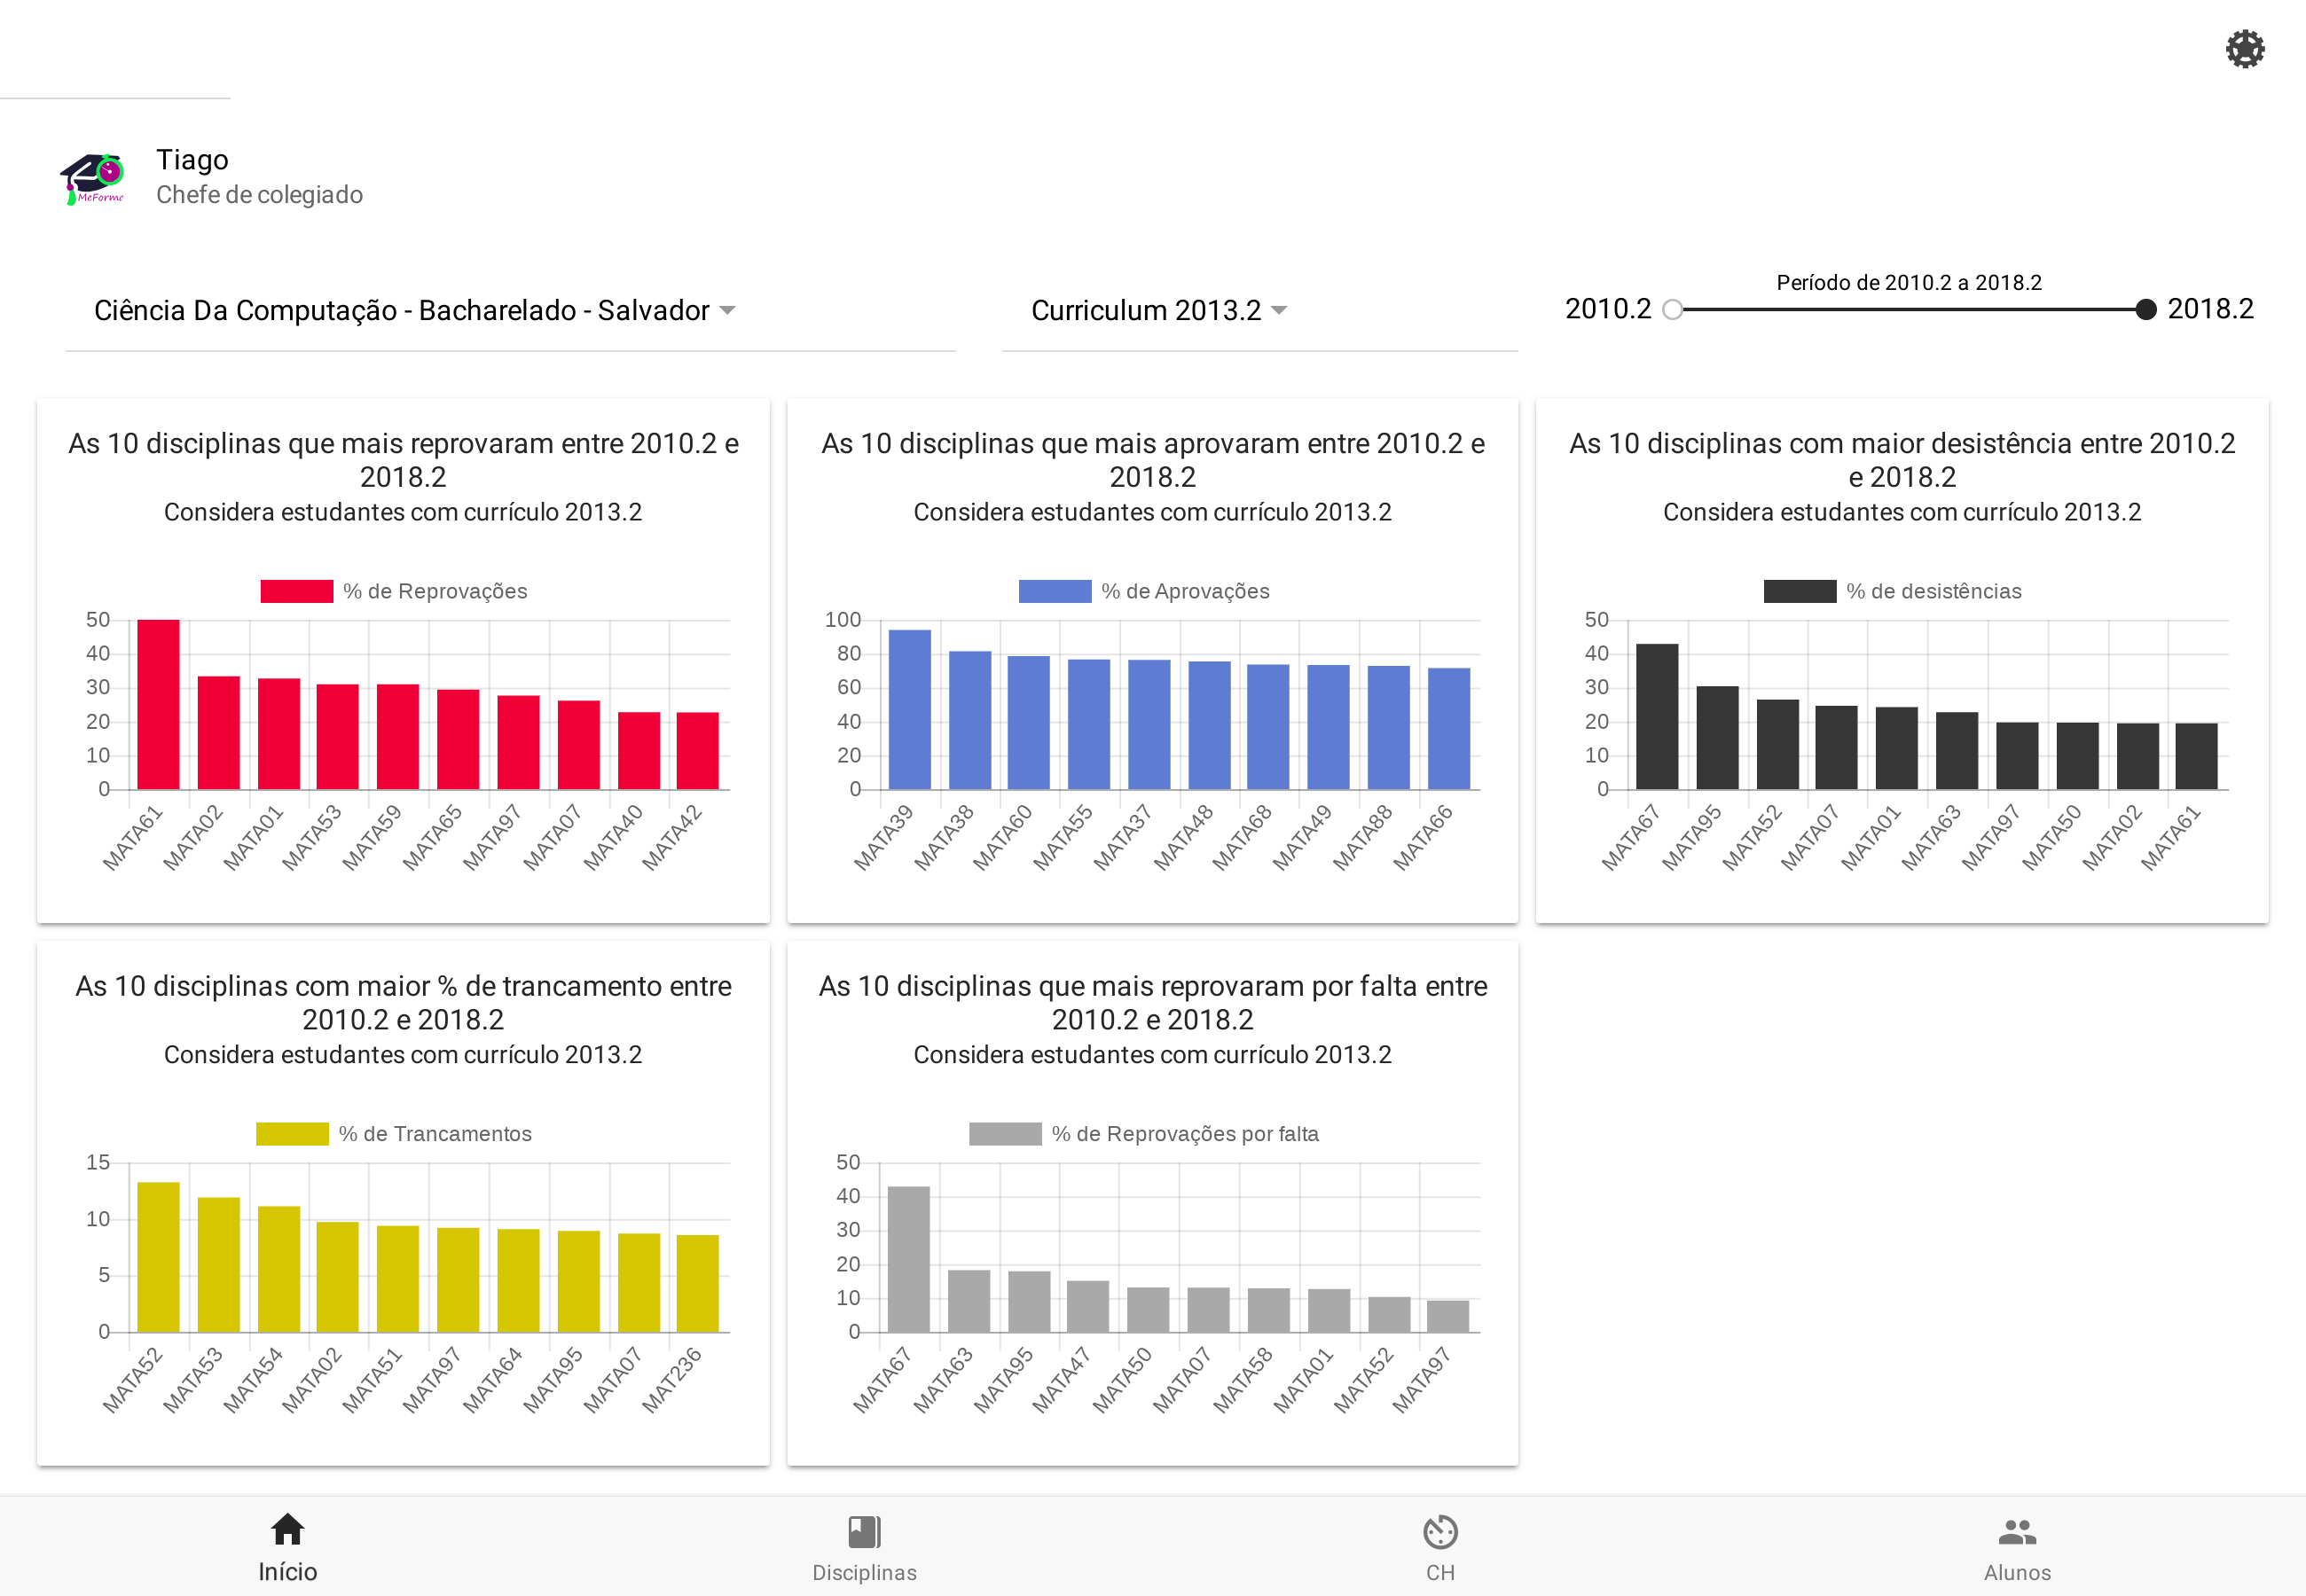
\includegraphics[scale=0.15]{pics/c3/15-charts.png}
	   \caption{Tela de resumo de desempenho nas disciplinas.}
	   \label{charts}
\end{figure}

\subsection{Lista de disciplinas do curso}

A tela de disciplinas do curso é semelhante em aparência àquela descrita na subsessão \ref{disciplinas_tela}, contudo, no MFPAC o objetivo é acompanhar o desempenho geral dos estudantes de um dado currículo em cada disciplina no decorrer do tempo. Para tal, além da porcentagem de aprovação de cada disciplina, quando o usuário clica em um cartão de disciplina, é exibido um gráfico que compara os percentuais de aprovação, reprovação, desistência, trancamento e reprovação por falta daquela disciplina. A Figura \ref{discipline-chart} exibe o desempenho dos estudantes do curso de Ciência da Computação da UFBA com currículo 2013.2 para o período de 2010.2 a 2018.2 na disciplina ``Compiladores''.

\begin{figure}[H]
	   \centering
	   		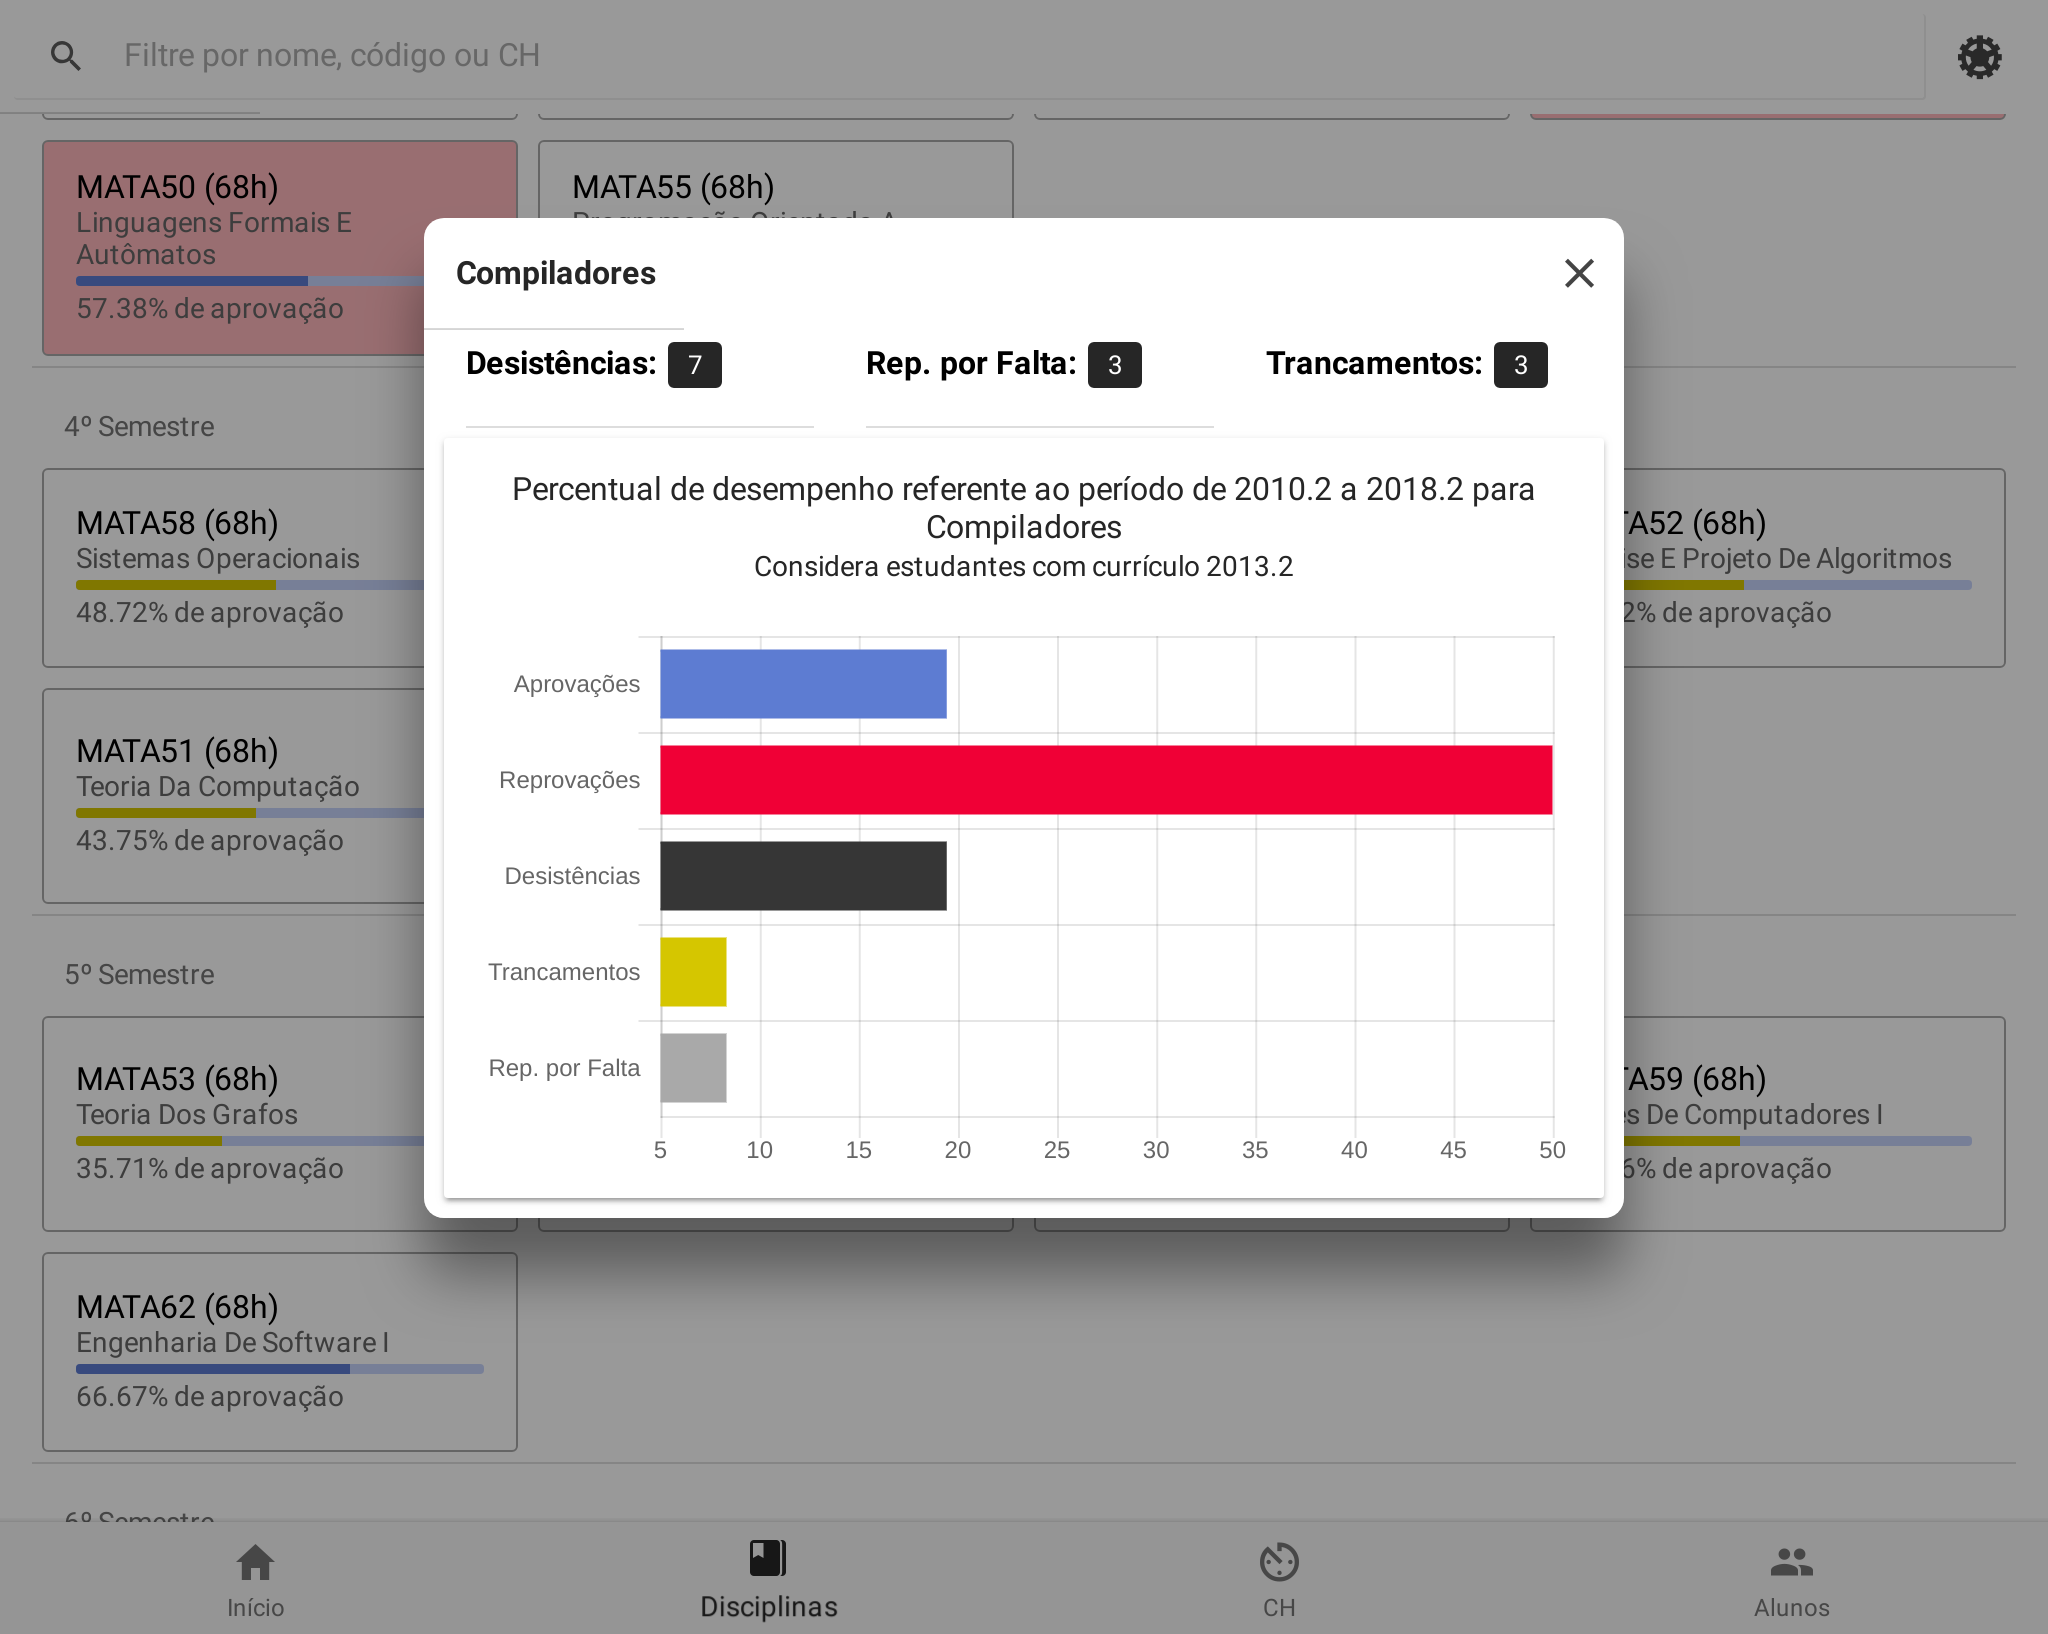
\includegraphics[scale=0.15]{pics/c3/16-compiladores.png}
	   \caption{Dados sobre a disciplina Compiladores.}
	   \label{discipline-chart}
\end{figure}

\subsection{Aproveitamentos de carga horária}

O objetivo dessa tela é exibir como os estudantes tem aproveitado carga horária para que o gestor possa principalmente dar indicações a alunos que precisam de carga horária. A Figura \ref{pacch} exibe a tela de aproveitamentos de carga horária.

\begin{figure}[H]
	   \centering
	   		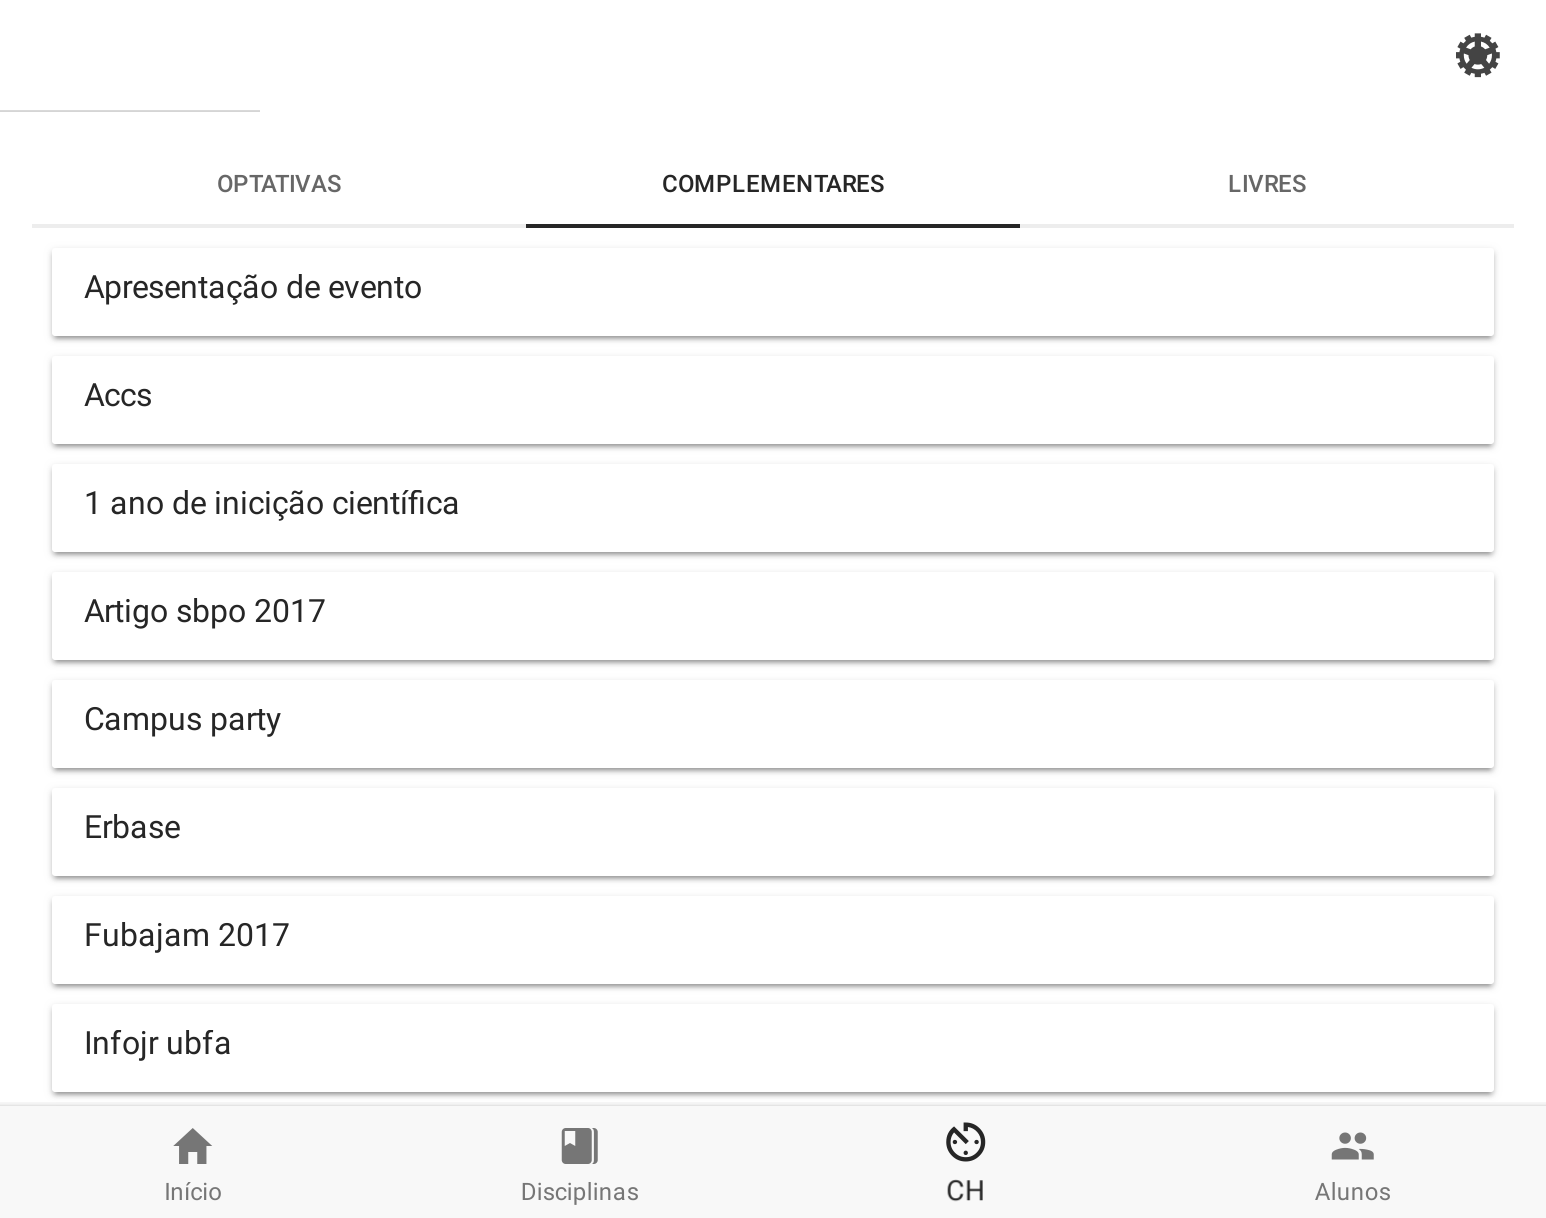
\includegraphics[scale=0.25]{pics/c3/17-ch.png}
	   \caption{Tela de aproveitamentos de carga horária.}
	   \label{pacch}
\end{figure}

\subsection{Listagem de estudantes}

A tela de listagem de estudantes tem o objetivo de exibir os estudantes que estão cadastrados no MeForma2 e os dados de curso dos mesmos, fornecendo ao gestor a quantidade de disciplinas que o estudante já cumpriu, a quantidade de carga horária que ele já proveitou e a quantidade mínima de semestres necessários para o estudante alcançar a formatura.

A quantidade mínima de semestres necessários para um estudante alcançar a formatura é calculada com base nas disciplinas obrigatórias que o mesmo ainda não cumpriu. Os demais requisitos para completude de um curso não foram incluídos no cálculo, pois a quantidade de horas que um aluno pode aproveitar em um semestre é imprevisível. A seguir é apresentado o algoritmo utilizado para determinar esse número.

\begin{enumerate}
    \item Subtrai-se o conjunto de disciplinas obrigatórias cursadas do conjunto de disciplinas obrigatórias total para obter o conjunto de disciplinas não cursadas.
    \item Contrói-se um grafo com as disciplinas não cursadas, onde cada disciplina é um vértice, a dependência entre elas são as arestas e o subgrafo formado por uma disciplina e suas dependências é uma árvore cuja altura determina a quantidade de semestres necessários para cumprir todas as disciplinas da árvore.
    \item A altura de cada árvore de disciplina é calculada e o valor da maior delas é armazenado.
    \item A moda da quantidade de disciplinas encaixadas em cada semestre do currículo do curso é calculada.
    \item A quantidade de disciplinas restantes é dividida pela moda calculada no passo 4 e armazenada.
    \item A quantidade de semestre necessários para cumprir as disciplinas obrigatórias restantes é dada pelo maior número entre o obtido no passo 3 e o obtido no passo 5.
\end{enumerate}

A Figura \ref{dgraph} exibe um grafo montado conforme o passo 2 para um usuário que precisa cumprir apenas as disciplinas MATA01, MATA02, MATA07, MATA65, MATA236 e FISA75. A maior altura de uma árvore para esse grafo é três (passo 3), e assumindo que a moda da quantidade de disciplinas por semestre é seis (passo 4), e como sete dividido por seis é menor do que três, a quantidade mínima de semestres necessárias para o aluno cumprir tais disciplinas é três. 

\begin{figure}[H]
	   \centering
	   		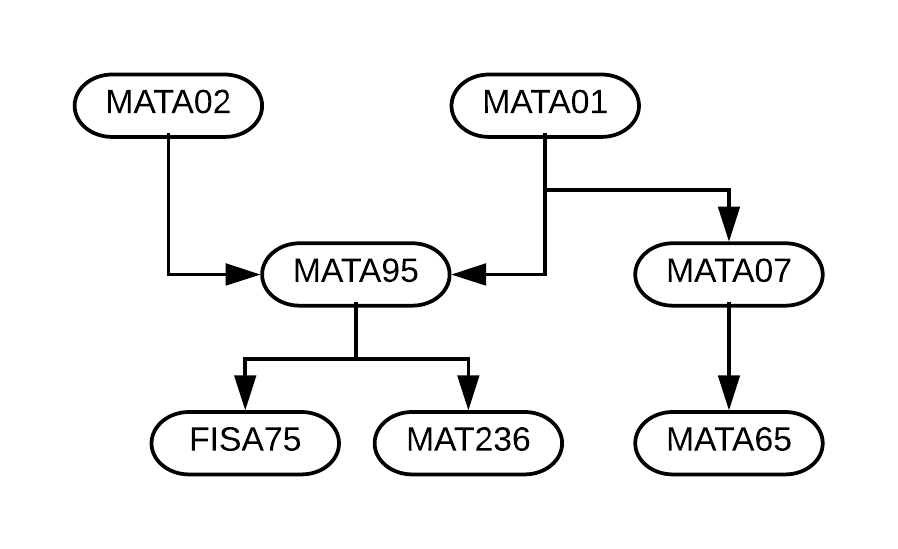
\includegraphics[scale=1.3]{pics/c3/19-graph.png}
	   \caption{Grafo de dependência entre as disciplinas restantes.}
	   \label{dgraph}
\end{figure}


A Figura \ref{students} exibe a tela de listagem de estudantes. Os dados pessoais que identificam o estudante foram propositalmente escondidos.  

\begin{figure}[H]
	   \centering
	   		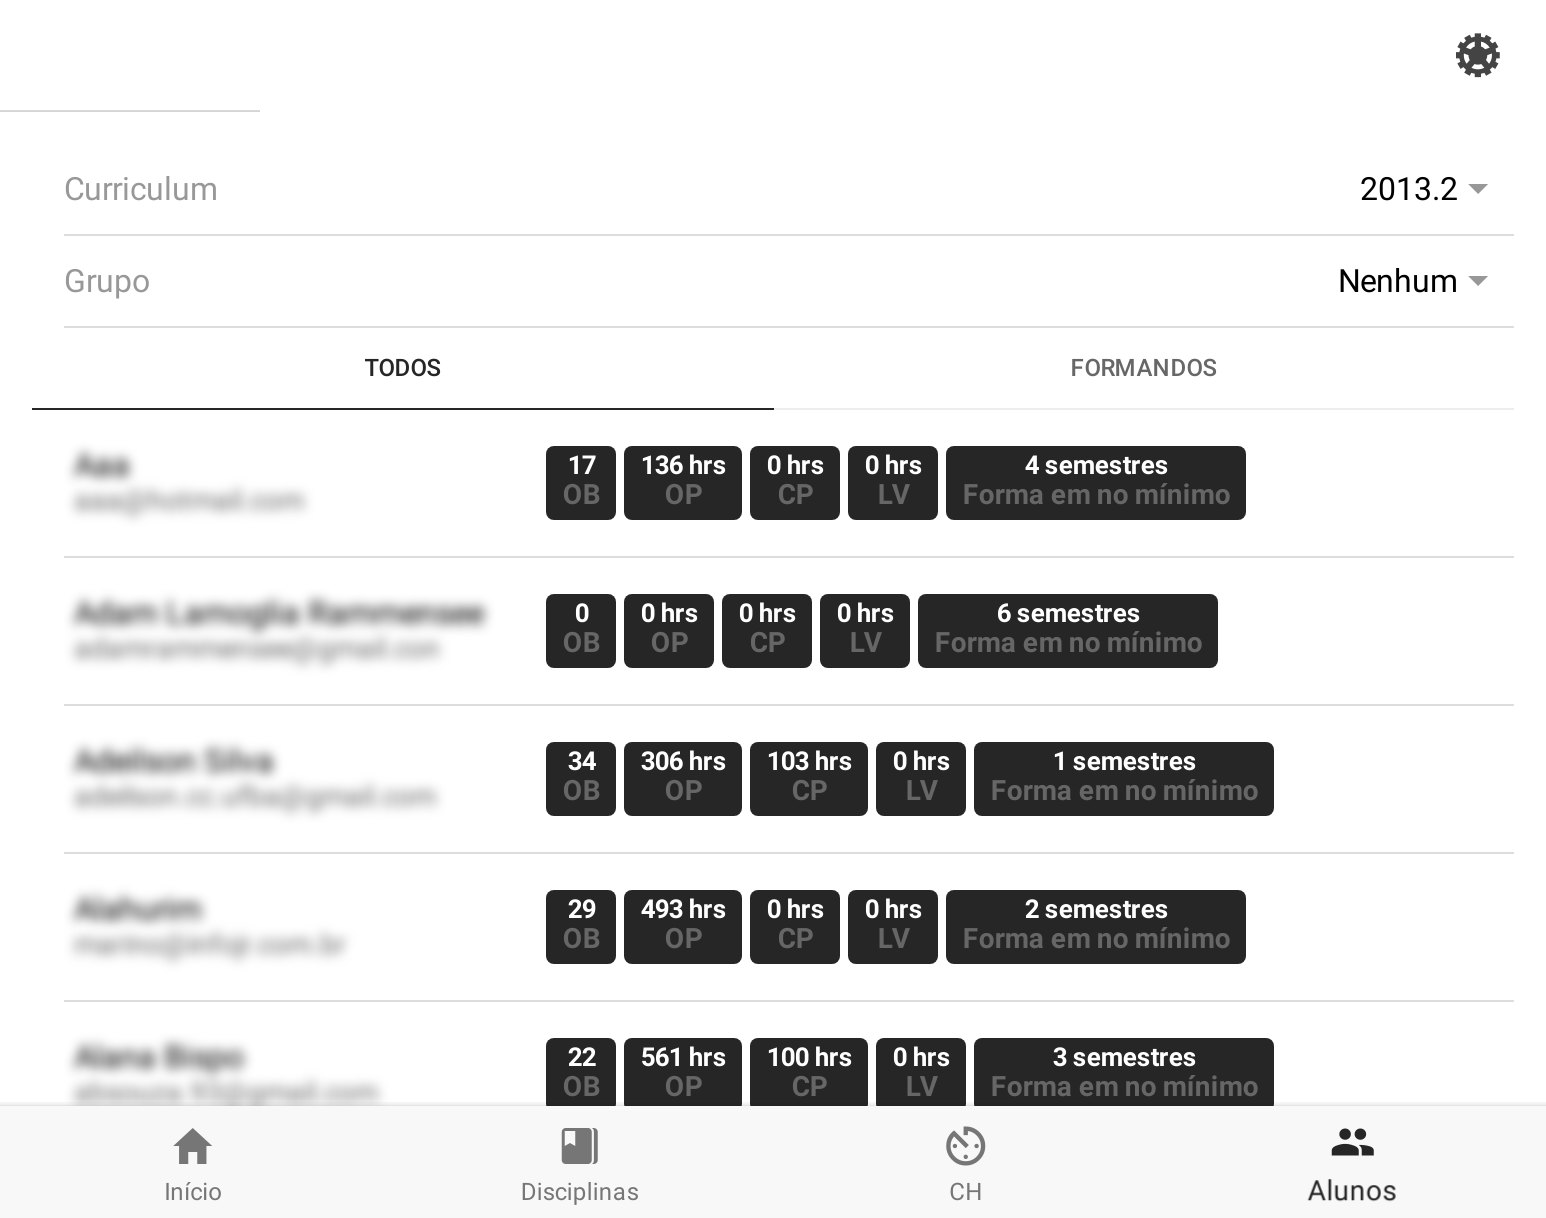
\includegraphics[scale=0.25]{pics/c3/18-students.png}
	   \caption{Tela de listagem de estudantes.}
	   \label{students}
\end{figure}


\section{Arquitetura do Aplicativo}
\label{frontend}
A seguir será apresentada a arquitetura do aplicativo, e a relação de comunicação entre as tecnologias que a compõem. Considerando como ponto de partida as tecnologias que estão em contato com o usuário, tecnicamente chamadas de ``Tecnologias FrontEnd'' até as tecnologias que estão funcionando em segundo plano no dispositivo do usuário.

\begin{figure}[H]
	   \centering
	   		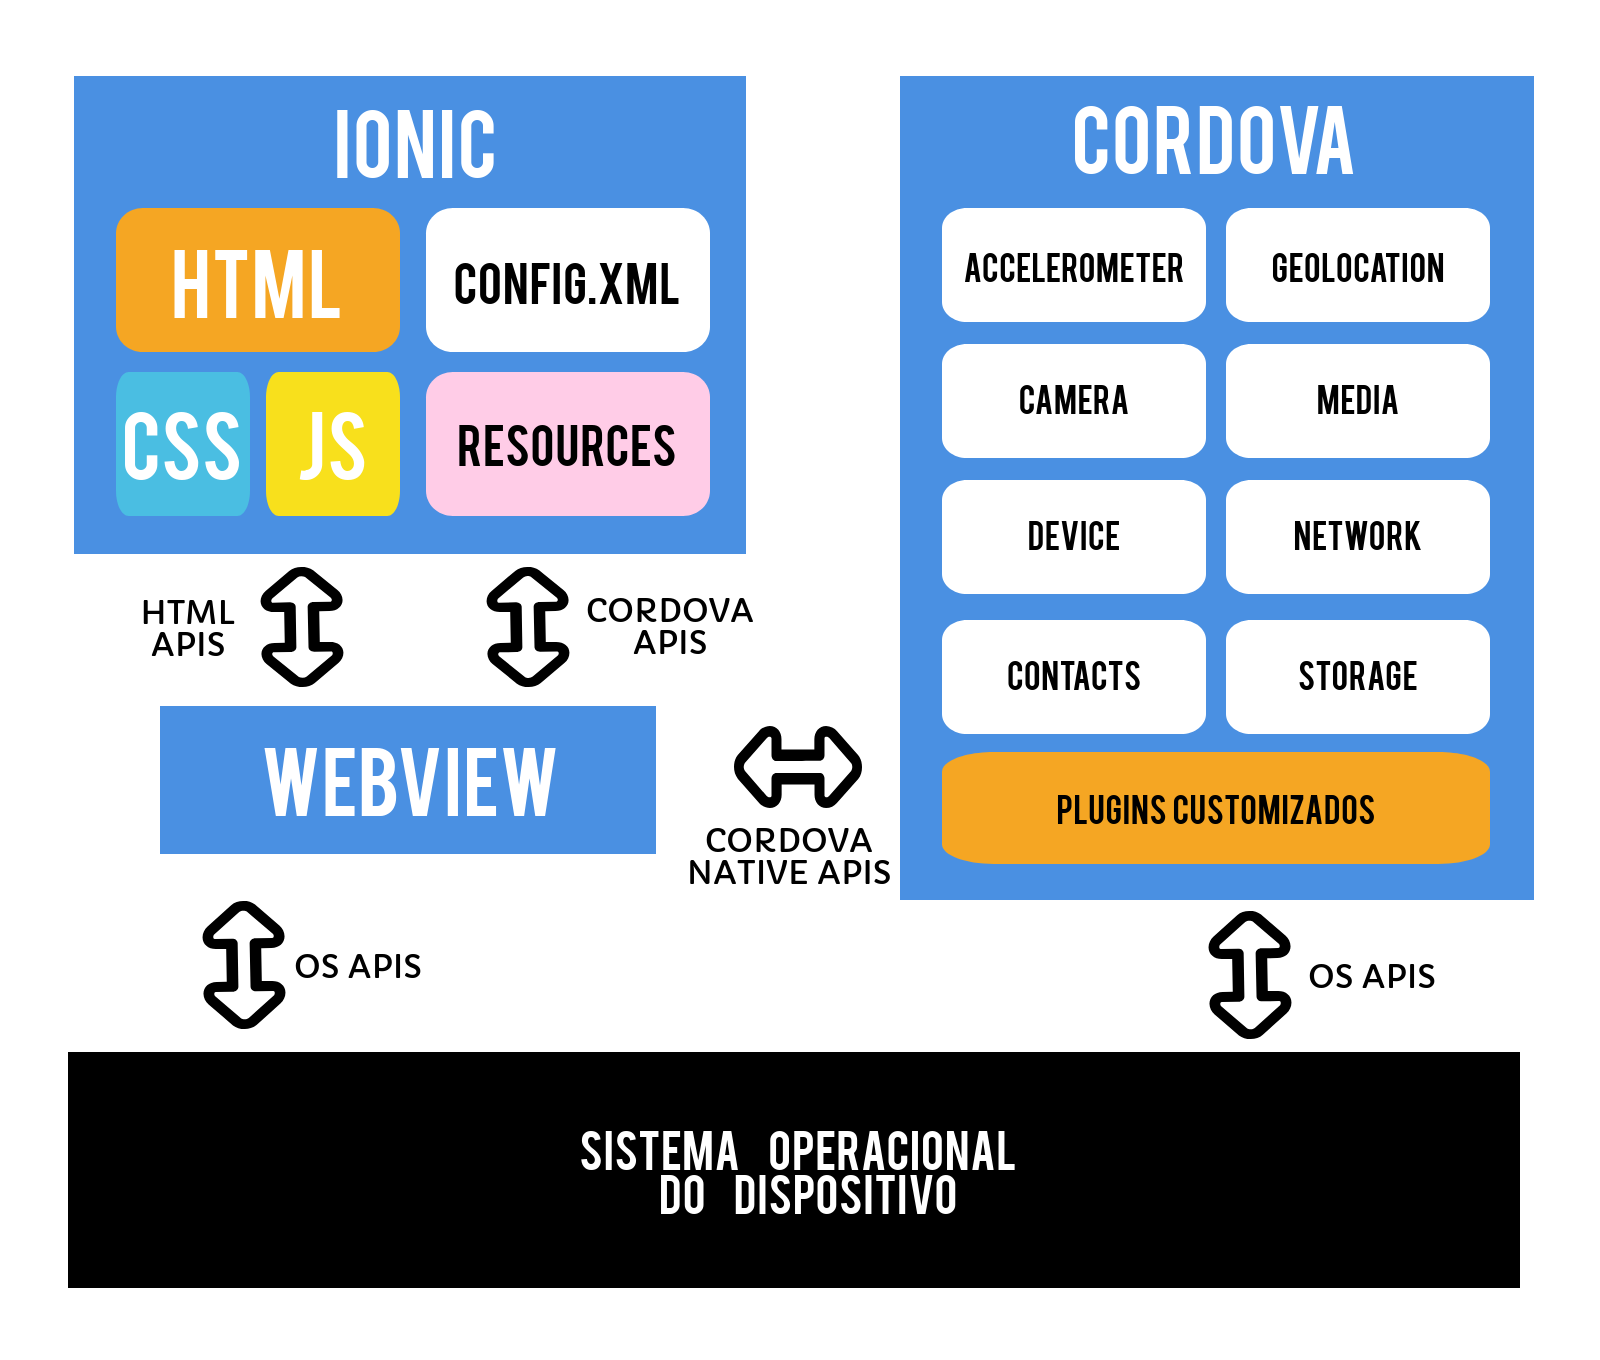
\includegraphics[scale=0.28]{pics/c3/0-arquitetura.png}
	   \caption{Arquitetura do Aplicativo}
	   \label{arquitetura}
\end{figure}

A figura~\ref{arquitetura} mostra a relação entre os componentes do aplicativo do MeForma2. Cada uma das caixas mais externas representa uma tecnologia. Cada seta na figura representa uma ponte de comunicação entre as tecnologias.

\section{Ionic Framework}

Com o Ionic Framework, ou simplismente Ionic, foi produzido o código fonte do aplicativo. Esse código fonte é dividido em 5 categorias de arquivos: HTML, CSS, JS, config.xml, e os resources que, no caso do MeForma são as imagens locais. Os arquivos HTML, CSS e JS são gerados após os pré-processadores cidatos na Seção~\ref{tecnologias} serem executados pelo Ionic.

O aplicativo é implementado como uma página da Web. Por padrão, um arquivo local chamado index.html faz referência ao CSS, JavaScript, imagens e outros recursos necessários para sua execução. O aplicativo é renderizado em um \textit{WebView} através da ponte de comunicação \textit{HTML APIs}.

Esse pacote tem ainda um arquivo config.xml que fornece informações sobre o aplicativo e especifica parâmetros que afetam como ele funciona, por exemplo, se o aplicativo deve responder às mudanças de orientação do dispositivo.

\subsection{WebView}

O \textit{WebView} é um componente do sistema operacional dos dispositivos móveis modernos para quando se quer entregar um aplicativo da Web como um aplicativo mobile ou como parte de um aplicativo. Seu funcionamento é semelhante ao de um navegador da Web, porém ele não inclui nenhum recurso de um navegador da Web totalmente desenvolvido, como controles de navegação ou uma barra de endereços. O que o WebView faz, por padrão, é executar e exibir uma página da web.

O WebView é capaz de estabelecer uma comunicação entre o conteúdo gerado pelo Ionic e o Cordova. E, quando a aplicação é executada num navegador da Web, é ele quem faz o papel do WebView.

\subsection{Cordova}

O Cordova é responsável por envolver o aplicativo em um contêiner com acesso às funções nativas do dispositivo em que o aplicativo está sendo executado. Essas funções são exposta via JavaScript para facilitar a integração com o aplicativo e com o WebView.

No código gerado pelo Ionic deve haver a informação de quais plugins do Cordova serão utilizados e de como deve ser essa utilização, então isso é solicitado do \textit{WebView} (Cordova APIs) que, por sua vez, solicita do Cordova (Cordova Native Apis).

\subsection{Sistema Operacional do Dispositivo}

O sistema operacional do dispositivo é o provedor dos recursos necessários para que o WebView e o Cordova possam utilizar o hardware do dispositivo do usuário.

\section{Arquitetura Lógica da Aplicação}

Esta seção descreve a arquitetura lógica do MeForma2. A aplicação foi desenvolvida utilizando o padrão de arquitetura de software \textit{Model–view–controller} (MVC). No MVC, o sistema é estruturado em três componentes lógicos que interagem entre si: Model, Controller e View.

\begin{itemize}
    \item O Model é o componente responsável pelo gerenciamento dos dados do sistema. Ele é o componente mais próximo do SGBD e seu papel no MeForma2 é realizar operações de leitura, atualização, criação e exclusão de dados.
    \item O Controller é o componente responsável pelas regras de negócio da aplicação e realiza tarefas de controle e tratamento de informações e dados.
    \item A View é o componente que define como as informações são apresentadas ao usuário.
\end{itemize}
\begin{figure}[H]
	   \centering
	   		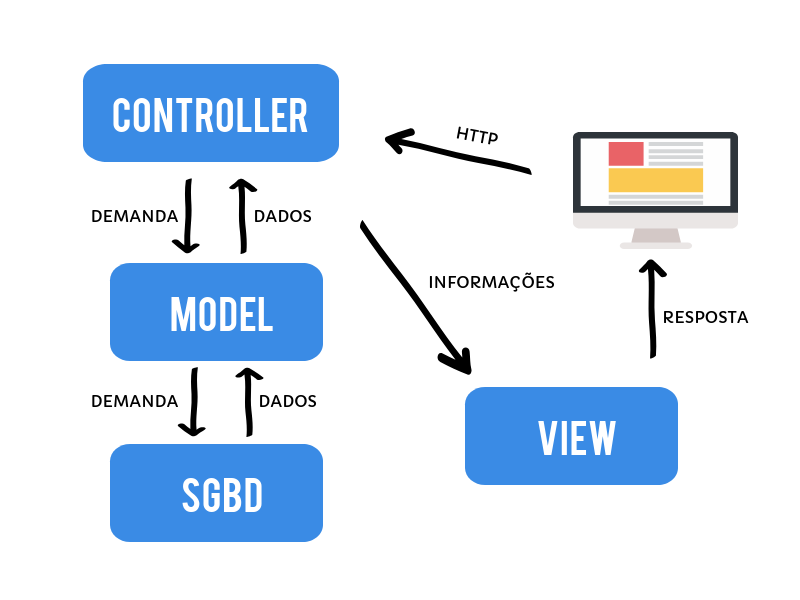
\includegraphics[scale=0.50]{pics/c3/12-mvc.png}
	   \caption{Representação conceitual do padrão MVC.}
	   \label{mvc}
\end{figure}
A Figura~\ref{mvc} mostra a relação entre os componentes do MVC e a conexão entre o MVC e o usuário (representado por um computador) que também pode ser interpretado como sendo o aplicativo. O usuário solicita um recurso do sistema através de uma requisição HTTP (padrão de comunicação utilizado na web), essa requisição é interpretada pelo Controller que a encapsula como uma demanda para o Model. Este, por sua vez, converte a demanda para um modelo de demanda do SGBD. O SGBD encaminha ao Model os dados correspondentes à demanda que recebeu, então o Model transforma os dados para um modelo que o Controller possa interpretar e os encaminha para ele. O Controller interpreta os dados recebidos do Model e os organiza para gerar informações, as quais são enviadas ao View que as padroniza para que sejam exibidas no dispositivo do usuário.

No MeForma2, os componentes do MVC são agrupados em um modelo de organização característico de aplicativos multiplataforma. Os componentes Controller e Model são agrupados em um pacote denominado API do inglês \textit{Application Programming Interface}.

A API do MeForma2 é responsável pela comunicação entre o aplicativo e o banco de dados. Por um lado, ela é a encarregada de transformar e controlar o conteúdo proveniente do Banco de Dados para que o aplicativo possa interpretar e exibir. No sentido oposto, ela é responsável por transformar os dados inseridos no aplicativo pelo usuário para que possam ser devidamente registrados no banco de dados.

\section{Banco de dados}

Essa seção justifica a estrutura adotada para armazenamento dos dados do MeForma2 em banco de dados.

\begin{figure}[H]
	   \centering
	   		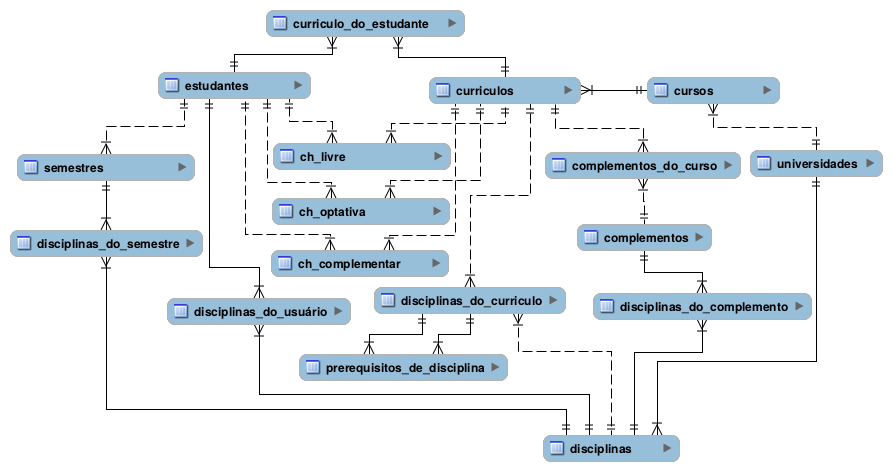
\includegraphics[scale=0.50]{pics/c3/4-db.png}
	   \caption{Diagrama de organização e relacionamento das tabelas}
	   \label{db}
\end{figure}

A Figura~\ref{db} mostra um diagrama de organização do banco de dados do MeForma2. A figura mostra como os dados do MeForma2 estão relacionados na estrutura de armazenamento.

Existem 3 tabelas principais no MeForma: a tabela ``estudantes'', a tabela ``currículos'' e a tabela ``disciplinas''. Elas estão no centro da aplicação e representam a região mais congestionada.

A estrutura pode ainda ser dividida em duas partes, a primeira composta pelas tabelas que dizem respeito aos dados que o sistema fornece ao usuário, que serão chamadas de ``tabelas do sistema'', e a segunda composta pelas tabelas que dizem respeito aos dados que o usuário fornece ao sistema, que serão chamadas de ``tabelas do usuário''.

\subsection{Tabelas do Sistema}
As tabelas que dizem respeito aos dados que o sistema fornece ao usuário são: ``universidades'', ``cursos'', ``currículos'', ``disciplinas'', ``disciplinas\_do\_currículo'', ``prerequisitos\_de\_disciplinas'', ``complementos'', ``complementos\_do\_curso'' e
``disciplinas\_do\_complemento''.

As tabelas ``universidades'' e ``cursos'' funcionam apenas como um filtro para o currículo. Todas as relações posteriores tratam de um estudante em seu currículo de curso ou de um currículo de curso e suas disciplinas.

É o currículo quem determina o tempo máximo e mínimo de formatura, a quantidade de carga horária que um estudante precisa cumprir e quais os tipos de carga horária que ele terá de cursar.

As disciplinas são associadas a uma universidade, e estão distribuídas entre os diversos currículos que estão associados aos cursos daquela universidade. Dessa forma, é possível obter diversas combinações de disciplinas para um mesmo curso. O que caracteriza parte de um currículo. A tabela ``disciplinas\_do\_curriculo'' gerencia quais disciplinas compõem cada currículo.

Uma disciplina pode ter, para cada currículo de curso, um conjunto de pré-requisitos. Por exemplo, os pré-requisitos para Álgebra Linear no currículo 2013.2 do curso de Ciência da Computação não são os mesmos para o currículo 2012.2 do curso de Sistemas de Informação. A tabela ``prerequisitos\_de\_disciplinas'' é responsável por gerenciar os pré-requisitos de cada disciplina em um currículo.

Alguns currículos oferecem a opção de especialização ou complemento para o estudante, e essa especialização ou complemento pode conter mais carga horária e mais disciplinas. Essa configuração é gerenciada pelas tabelas, ``complementos'', ``complementos\_do\_curso'' e ``disciplinas\_do\_complemento''.

\subsection{Tabelas do Usuário}

As tabelas que dizem respeito aos dados que o usuário fornece ao sistema são: `estudantes`, `currículo\_do\_estudante`, `ch\_complementar'', ``ch\_optativa'', ``ch\_livre'', ``semestres'', ``disciplinas\_do\_semestre'' e ``disciplinas\_do\_usuario''.

A tabela ``estudantes'' contém os dados que identificam um estudante no sistema, como por exemplo, nome e e-mail. A partir dessa tabela, a vida acadêmica do estudante começa a ser montada no MeForma2.

Todo estudante precisa se matricular em um currículo de curso, e essa informação é armazenada na tabela de ``currículo\_do\_estudante'', que é a primeira ponte entre as tabelas do sistema e as tabelas do usuário.

As demais tabelas são responsáveis pelos dados que resultam na porcentagem de conclusão de um determinado curso. As tabelas com prefixo ``ch\_'' são responsáveis por armazenar os aproveitamento de carga horária de cada estudante. A tabela disciplinas\_do\_usuário, armazena as disciplinas que cada estudante já concluiu. As tabelas ``semestres`` e ``disciplinas\_do\_semestre'' armazenam os semestres que cada estudante cursou e as disciplinas que compõem cada semestre para cada estudante.